\documentclass{report}
% ======================================================
% Encodage, langue et mise en page
% ======================================================
\usepackage[utf8]{inputenc}
\usepackage[T1]{fontenc}
\usepackage[french]{babel}
\usepackage[left=2cm,right=2cm,top=2cm,bottom=2cm]{geometry}

% ======================================================
% Mathématiques
% ======================================================
\usepackage{amsmath, amsfonts, amssymb, bm}
\setcounter{MaxMatrixCols}{10}

% ======================================================
% Graphiques, tableaux et couleurs
% ======================================================
\usepackage{graphicx}
\usepackage{float}
\usepackage{xcolor}
\usepackage{color}
\usepackage{array, multirow, makecell}
\usepackage{booktabs}
\usepackage{colortbl}
\usepackage{tabularx}
\usepackage{graphicx}
% ======================================================
% Boîtes, listes et symboles
% ======================================================
\usepackage{tcolorbox}
\usepackage{tikz}
\usetikzlibrary{positioning,arrows.meta,shapes.geometric}
\usepackage{fancybox}
\usepackage{pifont}
\usepackage{enumitem}
\usepackage{lipsum}
\usepackage{titlesec}
\usepackage{etoolbox}
\usepackage{xparse}
\usepackage[font=small,labelfont=bf,skip=2pt]{caption}
\captionsetup[figure]{position=top}
\captionsetup[table]{position=top}

\newcommand{\source}[1]{%
  \par\vspace{0.2\baselineskip}
  {\centering\footnotesize\itshape Source : #1\par}
}

\setlist[itemize]{leftmargin=1.5em, itemsep=2pt, parsep=0pt}
\setlist[enumerate]{leftmargin=1.8em, itemsep=2pt, parsep=0pt}
\setcounter{secnumdepth}{3}
\setcounter{tocdepth}{3}

% ======================================================
% Algorithmes
% ======================================================
\usepackage{algorithm}
\usepackage{algpseudocode}

% ======================================================
% Tables des matières
% ======================================================
\usepackage{shorttoc}
\usepackage{makeidx}

% ======================================================
% Théorèmes
% ======================================================
\newtheorem{theorem}{Théorème}[section]
\newtheorem{proposition}{Proposition}[section]
\newtheorem{definition}{Définition}[section]
\newtheorem{lemma}{Lemme}[section]
\newtheorem{corollary}{Corollaire}[section]
\newtheorem{property}{Propriétés}[section]
\newtheorem{example}{Exemple}[section]
\newtheorem{remark}{Remarque}[section]

% ======================================================
% Couleurs personnalisées
% ======================================================
\definecolor{lightblue}{rgb}{0.678, 0.847, 0.902}
\definecolor{darkblue}{RGB}{0,45,90}
\definecolor{midblue}{RGB}{0,90,160}
\definecolor{accentred}{RGB}{170,30,45}
\definecolor{bordeaux}{rgb}{.5,0,0}
\definecolor{kmeraiteal}{RGB}{0,137,151}
\definecolor{kmeraigreen}{RGB}{36,126,65}
\definecolor{kmeraired}{RGB}{196,34,48}
\definecolor{kmeraiorange}{RGB}{242,151,0}
\definecolor{kmeraigray}{RGB}{65,65,65}

\setlist[itemize,1]{
  label=\textcolor{kmeraiteal}{\ding{228}},
  leftmargin=1.8em,
  itemsep=2pt,
  parsep=0pt
}
\setlist[itemize,2]{
  label=\textcolor{kmeraigreen}{\ding{226}},
  leftmargin=1.6em,
  itemsep=1pt,
  parsep=0pt
}
\setlist[itemize,3]{
  label=\textcolor{kmeraiorange}{\scriptsize\ding{108}},
  leftmargin=1.4em,
  itemsep=1pt,
  parsep=0pt
}

% Couleurs des titres inspirees de l'identite visuelle KmerAI
\titleformat{\section}
  {\normalfont\Large\bfseries\color{kmeraiteal}}
  {\thesection}{0.8em}{}
\titleformat{\subsection}
  {\normalfont\large\bfseries\color{kmeraigreen}}
  {\thesubsection}{0.8em}{}
\titleformat{\subsubsection}
  {\normalfont\normalsize\bfseries\color{kmeraired}}
  {\thesubsubsection}{0.8em}{}
\titlespacing*{\section}{0pt}{1.2ex plus .2ex}{0.8ex}
\titlespacing*{\subsection}{0pt}{1ex plus .2ex}{0.6ex}
\titlespacing*{\subsubsection}{0pt}{0.8ex plus .2ex}{0.5ex}

% ======================================================
% Commandes personnalisées
% ======================================================
\newcommand{\R}{\mathbb{R}}
\newcommand{\N}{\mathbb{N}}
\renewcommand{\vec}[1]{\bm{#1}}
\newcommand{\mat}[1]{\mathbf{#1}}
\newcommand{\softmax}{\operatorname{softmax}}

\newcommand{\BERT}{\textsc{bert}}
\newcommand{\GPT}{\textsc{gpt}}
\newcommand{\ESCO}{\textsc{esco}}
\newcommand{\NCM}{\textsc{ncm}}
\newcommand{\MEPC}{\textsc{mepc}}
\newcommand{\NCF}{\textsc{ncf}}
\newcommand{\RAG}{\textsc{rag}}
\newcommand{\KG}{\textsc{kg}}
\newcommand{\GCN}{\textsc{gcn}}
\newcommand{\GAT}{\textsc{gat}}
\newcommand{\GNN}{\textsc{gnn}}
\newcommand{\LLM}{\textsc{llm}}

\def\dessous#1\sous#2{\mathrel{\mathop{\kern0pt#2}\limits_{#1}}}

% ======================================================
% Style tcolorbox
% ======================================================
\tcbset{
  formulabox/.style={
    colback=blue!3,
    colframe=midblue,
    boxrule=0.7pt,
    arc=2mm,
    left=2mm,
    right=2mm,
    top=1mm,
    bottom=1mm
  },
  figplaceholder/.style={
    colback=blue!3,
    colframe=midblue,
    boxrule=0.7pt,
    arc=2mm,
    left=2mm,
    right=2mm,
    top=2mm,
    bottom=2mm
  },
  figurebox/.style={
    colback=white,
    colframe=kmeraiteal,
    boxrule=0.9pt,
    arc=1.5mm,
    hbox,
    left=2mm,
    right=2mm,
    top=2mm,
    bottom=2mm
  }
}

\newif\iffiguregraphicbox
\AtBeginEnvironment{figure}{\figuregraphicboxtrue}
\AtEndEnvironment{figure}{\figuregraphicboxfalse}

\let\originalincludegraphics\includegraphics
\RenewDocumentCommand{\includegraphics}{s O{} m}{%
  \iffiguregraphicbox
    \par\noindent\makebox[\textwidth][c]{%
      \begin{tcolorbox}[figurebox]
        \IfBooleanTF{#1}
          {\originalincludegraphics*[#2]{#3}}
          {\originalincludegraphics[#2]{#3}}
      \end{tcolorbox}%
    }\par\vspace{-0.15\baselineskip}%
  \else
    \IfBooleanTF{#1}
      {\originalincludegraphics*[#2]{#3}}
      {\originalincludegraphics[#2]{#3}}%
  \fi
}

% Encadré formule numérotée
\newenvironment{formule}[1][]{%
  \begin{tcolorbox}[formulabox]
  \begin{equation}
}{%
  \end{equation}
  \end{tcolorbox}
}

% ======================================================
% Mise en forme générale
% ======================================================
\frenchspacing
\linespread{1.4}
\raggedbottom
\oddsidemargin -0.2cm
\evensidemargin 0cm
\textheight 24cm
\textwidth 16cm
\voffset -0.5cm
\setlength{\headsep}{0.35cm}

% ======================================================
% Personnalisation des chapitres
% ======================================================
\makeatletter

\newcommand{\thechapterwords}{%
  \ifcase \value{chapter}
  \or 1
  \or 2
  \or 3
  \or 4
  \or 5
  \or Six
  \or Seven
  \or Eight
  \or Nine
  \or Ten
  \or Eleven
  \fi
}

\def\thickhrulefill{%
  \leavevmode
  \leaders \hrule height 1ex \hfill
  \kern \z@
}

\def\@makechapterhead#1{%
  \vspace*{15\p@}
  {\parindent \z@ \centering \reset@font
    \thickhrulefill\quad
    \scshape\@chapapp{} \thechapterwords
    \quad \thickhrulefill
    \par\nobreak
    \vspace*{10\p@}
    \interlinepenalty\@M
    \hrule
    \vspace*{10\p@}
    \Huge \bfseries #1\par\nobreak
    \par
    \vspace*{10\p@}
    \hrule
    \vskip 60\p@
  }
}

\def\@makeschapterhead#1{%
  {\parindent \z@ \centering \reset@font
    \thickhrulefill
    \par\nobreak
    \vspace*{10\p@}
    \interlinepenalty\@M
    \hrule
    \vspace*{10\p@}
    \Huge \bfseries #1\par\nobreak
    \par
    \vspace*{10\p@}
    \hrule
    \vskip 60\p@
  }
}

\makeatother

% ======================================================
% En-têtes et pieds de page
% ======================================================
\usepackage{fancyhdr}

\pagestyle{fancy}
\fancyhf{}
\renewcommand{\chaptermark}[1]{\markboth{#1}{#1}}
\renewcommand{\sectionmark}[1]{\markright{#1}}
\fancyhead[L]{\textsl{\nouppercase{\rightmark}}}
\fancyfoot[L]{NGOULOU NGOUBILI Irch Defluviaire}
\fancyfoot[C]{\textbf{\thepage}}
\fancyfoot[R]{Memoire Professionnel}
\renewcommand{\headrulewidth}{1pt}
\renewcommand{\footrulewidth}{0.5pt}
\addtolength{\headheight}{1pt}

\fancypagestyle{plain}{%
  \fancyhead{}
  \fancyfoot[L]{NGOULOU NGOUBILI Irch Defluviaire}
  \fancyfoot[C]{\textbf{\thepage}}
  \fancyfoot[R]{Memoire Professionnel}
  \renewcommand{\headrulewidth}{0pt}
  \renewcommand{\footrulewidth}{0.5pt}
}

\newcommand{\clearemptydoublepage}{%
  \newpage{\pagestyle{plain}\cleardoublepage}
}

% ======================================================
% Bibliographie : citations numériques [1], [2], ...
% ======================================================
\usepackage[
  backend=biber,
  style=numeric,
  sorting=none
]{biblatex}

\addbibresource{references.bib}

% ======================================================
% Hyperliens — à charger après biblatex
% ======================================================
\usepackage[
  colorlinks=true,
  linkcolor=darkblue,
  citecolor=midblue,
  urlcolor=accentred,
  bookmarks=true,
  bookmarksopen=true
]{hyperref}


\begin{document}

\begin{titlepage}
\begin{tikzpicture}[remember picture, overlay]
  \draw[midblue, line width=3pt]
    ([xshift=1cm, yshift=-1cm]current page.north west)
    rectangle
    ([xshift=-1cm, yshift=1cm]current page.south east);
\end{tikzpicture}

\vspace*{0.45cm}
\noindent
\begin{minipage}[t]{0.47\textwidth}
   \begin{center}
\textit{\textbf{Communauté Économique et Monétaire de l'Afrique Centrale}}\\
 (CEMAC)\\[.15cm]

\includegraphics[scale=0.1037]{figures/40ansISSEA.png}
 \end{center}
\begin{center}
\textit{\textbf{Institut Sous-régional de Statistique\\  
		 et d'Économie Appliquée}}\\[0.18cm]
{\underline{\textit{\textbf{Organisation Internationale}}}}\\
BP : 294 Yaoundé - Tél : 222 220 134 
\end{center}
 \end{minipage}\hfill
\begin{minipage}[t]{0.47\textwidth}
   \begin{center}
\textit{\textbf{Cameroun AI Enthousiaste}}\\[0.16cm]

\includegraphics[scale=0.73]{figures/kmerai.png}
 \end{center}
\begin{center}
\textit{\textbf{Direction du Développement et de la Recherche}}\\[0.16cm]
	{\underline{\textit{\textbf{ONG camerounaise}}}}\\
BP : 83000 Toulon, France
\end{center}
 \end{minipage}
\vspace*{0.2cm}
\begin{center}
	\large {\textbf{\textit{Mémoire professionnel de fin d’étude présenté en vue de l’obtention du diplôme d’Ingénieur
Statisticien Économiste(ISE)}}}\\[0.2cm] 
	\large{\textbf{\textit{\underline{OPTION :} Data Science et Marketing}}}
\\[0.2cm]
%\includegraphics[scale=0.7]{sty.png}\\
    % Title
    {\color{midblue}\rule[-0.002mm]{17cm}{2.2mm}} \\[0.0001cm]\definecolor{bordeaux}{rgb}{.5,0,0}%Modélisation d'un système de recommandation hybride basé sur les Graphes de connaissances
    \Large \textbf{\color{blue!100!black}{CONCEPTION D'UN SYSTEME DE RECOMMANDATION HYBRIDE POUR LE MATCHING EMPLOI-COMPETENCES AU CAMEROUN PAR INTEGRATION DES LLMS ET DES GRAPHES DE CONNAISSANCES}}
    {\color{midblue}\rule[-0.002mm]{17cm}{2.2mm}}\definecolor{bordeaux}{rgb}{.4,0,0}
\par\vspace{0.8mm}
   \tcbox[colback=blue!4, colframe=midblue, boxrule=0.8pt, arc=1mm, left=2mm, right=2mm, top=0.8mm, bottom=0.8mm]{\textbf{\small Rédigé par :}}\par\vspace{0.8mm}
    {\large\bfseries NGOULOU NGOUBILI Irch Defluviaire}\\
    {\normalsize Élève Ingénieur Statisticien Économiste cycle long -- $5^e$ année}\\[0.12cm]
    \tcbox[colback=blue!4, colframe=midblue, boxrule=0.8pt, arc=1mm, left=2mm, right=2mm, top=0.8mm, bottom=0.8mm]{\textbf{\small Sous l'encadrement de :}}\par\vspace{0.2cm}
    {\large\bfseries Dr. FOUTSE Yuehgoh}\\
    {\normalsize Présidente \& Directrice exécutive adjointe, PhD Computer Science \& Data Scientist}
\end{center}
 \begin{center}
    \tcbox[colback=midblue, colframe=midblue, boxrule=0.8pt, arc=1mm, left=3mm, right=3mm, top=1mm, bottom=1mm]{\large\textbf{\textcolor{white}{Année académique 2025-2026}}}
  \end{center}
\end{titlepage}

\pagenumbering{roman}

\chapter*{Dédicace}
\markboth{Dédicace}{Dédicace}
\addcontentsline{toc}{chapter}{Dédicace}
\begin{flushright}
    \textit{À mes parents... (Max 1 page)}
\end{flushright}


\chapter*{Remerciements}
\markboth{Remerciements}{Remerciements}
\addcontentsline{toc}{chapter}{Remerciements}


\markboth{Sommaire}{Sommaire}
\shorttableofcontents{Sommaire}{1} % Pour le sommaire

%\chapter*{Sommaire} % Sommaire court (Guide 2.5)
%\begin{spacing}{1}
%    \@starttoc{toc}
%\end{spacing}


\chapter*{Liste des sigles et abréviations}
\markboth{Liste des sigles et abréviations}{Liste des sigles et abréviations}
\addcontentsline{toc}{chapter}{Liste des sigles et abréviations}

\vspace{-0.8cm}
{\footnotesize
\renewcommand{\arraystretch}{0.86}
\noindent\begin{tabularx}{\textwidth}{@{}p{2.5cm}X@{}}
ANN : & Approximate Nearest Neighbors \\
API : & Application Programming Interface \\
BERT : & Bidirectional Encoder Representations from Transformers \\
BI : & Business Intelligence \\
CEMAC : & Communauté Économique et Monétaire de l'Afrique Centrale \\
CV : & Curriculum Vitae \\
DCG : & Discounted Cumulative Gain \\
ESCO : & European Skills, Competences, Qualifications and Occupations \\
FAISS : & Facebook AI Similarity Search \\
FNE : & Fonds National de l'Emploi \\
FRED : & Federal Reserve Economic Data \\
GAT : & Graph Attention Network \\
GCN : & Graph Convolutional Network \\
GNN : & Graph Neural Network \\
GPT : & Generative Pre-trained Transformer \\
GPU : & Graphics Processing Unit \\
HNSW : & Hierarchical Navigable Small World \\
IA : & Intelligence Artificielle \\
IDCG : & Ideal Discounted Cumulative Gain \\
ISE : & Ingénieur Statisticien Économiste \\
ISSEA : & Institut Sous-régional de Statistique et d'Économie Appliquée \\
IVF : & Inverted File Index \\
KG : & Knowledge Graph \\
LLM : & Large Language Model \\
LoRA : & Low-Rank Adaptation \\
LSTM : & Long Short-Term Memory \\
MAP : & Mean Average Precision \\
MEPC : & Nomenclature Camerounaise des Métiers, Emplois et Professions \\
MRR : & Mean Reciprocal Rank \\
NCF : & Nomenclature Camerounaise des Formations \\
NCM : & Nomenclature Camerounaise des Métiers \\
NDCG : & Normalized Discounted Cumulative Gain \\
NLP : & Natural Language Processing \\
OIT : & Organisation Internationale du Travail \\
ONG : & Organisation Non Gouvernementale \\
QLoRA : & Quantized Low-Rank Adaptation \\
RAG : & Retrieval-Augmented Generation \\
RNN : & Recurrent Neural Network \\
RWKV : & Receptance Weighted Key Value \\
SEO : & Search Engine Optimization \\
SGPT : & Sentence Generative Pre-trained Transformer \\
SQL : & Structured Query Language \\
SR : & Système de Recommandation \\
\end{tabularx}
}

\vspace{0.2cm}

\listoftables
\markboth{Liste des tableaux}{Liste des tableaux}
\addcontentsline{toc}{chapter}{Liste des tableaux}

\listoffigures
\markboth{Liste des figures}{Liste des figures}
\addcontentsline{toc}{chapter}{Liste des figures}


\chapter*{Avant-propos}
\markboth{Avant-propos}{Avant-propos}
\addcontentsline{toc}{chapter}{Avant-propos}
% Présenter l'ISSEA et ses missions ici.
\vspace{-1.4cm}
L’Institut Sous-régional de Statistique et d’Économie Appliquée (ISSEA), institution spécialisée de la CEMAC créée en 1984, a pour mission principale la formation de cadres supérieurs en statistique, économie et data science, capables de répondre aux enjeux contemporains de décision fondée sur les données. Dans ce cadre, l’ISSEA propose plusieurs filières de formation, parmi lesquelles figure celle des Ingénieurs Statisticiens Économistes (ISE), alliant rigueur mathématique, modélisation économétrique et outils modernes d’analyse de données (Data Science).

Arrivés à un niveau avancé de leur formation, les élèves Ingénieurs Statisticiens Économistes sont tenus d’effectuer un stage professionnel d’une durée minimale de trois (03) mois. Ce stage constitue une phase essentielle du cursus, permettant de confronter les connaissances théoriques acquises à des problématiques réelles, tout en favorisant l’acquisition de compétences opérationnelles en environnement professionnel. Il est sanctionné par la rédaction d’un mémoire professionnel, soutenu devant un jury.

C’est dans ce cadre que nous avons effectué un stage du 9 mars 2026 au 30 juin 2026 au sein de KmerAI, où nous avons été intégrés à la Direction du Développement et de la Recherche. Cette immersion nous a permis de travailler sur une problématique appliquée située au croisement de l’analyse de données, de l’intelligence artificielle générative, du traitement automatique du langage naturel et de l’aide à la décision : l’amélioration du matching entre offres d’emploi, profils de candidats et compétences recherchées sur le marché camerounais.

Le présent mémoire s’inscrit dans cette dynamique et porte sur le thème : « Conception d’un système de recommandation hybride pour le matching emploi-compétences au Cameroun par intégration des
LLMs et des graphes de connaissances ». Il vise principalement à concevoir une architecture capable de structurer les données d’offres et de profils, d’exploiter les référentiels métiers et formations, puis de produire des recommandations plus explicables que les approches fondées uniquement sur des mots-clés. Plus spécifiquement, il s’agit de normaliser les données disponibles, d’aligner les métiers et compétences avec les référentiels \ESCO{}, \MEPC{} et \NCF{}, d’adapter un modèle d’embeddings au domaine emploi-compétences, de construire un graphe de connaissances sous Neo4j et de poser les bases d’un moteur de recommandation hybride intégrant similarité sémantique, relations de graphe et analyse du \emph{skill gap}.

Ce travail répond à un double enjeu. Sur le plan scientifique et méthodologique, il cherche à montrer comment les modèles de représentation sémantique, les bases vectorielles et les graphes de connaissances peuvent être combinés pour traiter un problème réel d’appariement sur le marché du travail. Sur le plan opérationnel, il propose une démarche reproductible susceptible d’aider KmerAI à développer des outils de recommandation, d’orientation et de montée en compétences adaptés aux besoins des candidats, des recruteurs et des acteurs de la formation.

\chapter*{Résumé}
\markboth{Résumé}{Résumé}
\addcontentsline{toc}{chapter}{Résumé}
% Contexte, problématique, méthode, résultats clés (Max 250 mots).
\vspace{-1.4cm}


\vfill  % Pour liberer un peu d'espace
\textbf{Mots-clés :} Économétrie, Statistique, Développement...


\chapter*{Abstract}
\markboth{Abstract}{Abstract}
\addcontentsline{toc}{chapter}{Abstract}
% Version anglaise du résumé.
\vspace{-1.4cm}



%=======================================================
% 3. CORPS DU DOCUMENT (Chiffres arabes)
% ======================================================
\newpage
\pagenumbering{arabic}







\chapter*{INTRODUCTION GÉNÉRALE}
\markboth{Introduction générale}{Introduction générale}
\addcontentsline{toc}{chapter}{Introduction générale}
% Contexte, Problématique, Objectifs, Hypothèses, Méthodologie, Plan.
\vspace{-1.4cm}
\section*{Contexte et justification}
\markright{Contexte et justification}
Le fonctionnement du marché de l'emploi constitue un déterminant central de la performance économique et sociale d’un pays. Au Cameroun, ce marché reste marqué par des déséquilibres structurels persistants, notamment l’inadéquation entre les compétences disponibles et les besoins des entreprises, la forte informalité et les difficultés d’insertion professionnelle des jeunes. Les données disponibles montrent que le chômage des jeunes demeure une réalité importante, avec un taux estimé à 6,6\% en 2024 et 6,5\% en 2025 selon les estimations modélisées de l’OIT relayées par la Banque Mondiale et la base FRED.Par ailleurs, plusieurs travaux sur le Cameroun soulignent que le problème ne tient pas uniquement au manque d’emplois, mais aussi à un mismatch entre formation, compétences et exigences du marché.
\par Dans ce contexte, la question du matching emploi-compétences devient centrale. En théorie, un marché du travail efficient devrait permettre d’associer rapidement les profils disposant des compétences requises aux postes vacants correspondants. En pratique, plusieurs frictions informationnelles persistent : asymétrie d’information entre recruteurs et candidats, faible structuration des profils de compétences, hétérogénéité des offres d’emploi et faiblesse des systèmes d’intermédiation comme le FNE et certains agences de recrutement. Ces dysfonctionnements conduisent à une situation paradoxale où coexistent des postes non pourvus et des chercheurs d’emploi, traduisant une inefficacité allocative du marché du travail.

Par ailleurs, l’essor des technologies numériques et de l’intelligence artificielle ouvre des perspectives nouvelles pour améliorer l’appariement entre offres et profils. Dans cette dynamique, KmerAI se positionne comme une plateforme camerounaise dédiée à la promotion de l’intelligence artificielle, à la vulgarisation de ses usages et à l’accompagnement des étudiants, chercheurs et entreprises dans l’adoption de solutions innovantes adaptées au contexte local. Ses missions consistent notamment à former aux bases de l’IA, à offrir un espace de partage d’expériences et à encourager la collaboration autour de cas d’usage appliqués à des secteurs stratégiques tels que la santé, l’agriculture, le transport, l’éducation et le marketing.

Cette orientation est particulièrement pertinente pour le marché de l’emploi camerounais, où les données liées aux offres, aux CV et aux compétences restent souvent dispersées et peu exploitées. Une approche fondée sur l’intelligence artificielle peut permettre d’analyser plus efficacement ces données hétérogènes afin de proposer des recommandations d’emploi plus pertinentes, plus rapides et plus personnalisées.
\vspace{-0.5cm}
\section*{Problématique}
\markright{Problématique}
Le marché de l'emploi camerounais est marqué par une forte asymétrie d'information, 
une hétérogénéité des profils professionnels et des offres d'emploi, ainsi qu'une 
faible capacité des outils classiques à évaluer les écarts réels de compétences. 
Les systèmes fondés sur des mots-clés ou des filtres statiques ne parviennent pas 
à détecter les compétences implicites, les équivalences sémantiques et les trajectoires 
de montée en compétences.

Par ailleurs, si des référentiels structurants existent notamment la Nomenclature Camerounaise des Métiers (NCM 2013), le référentiel européen \ESCO{} et la Nomenclature Camerounaise des Formations (\NCF{}), leur intégration opérationnelle dans les plateformes et outils d'appariement reste encore limitée. Ils sont peu exploités pour aligner les intitulés locaux de métiers sur des standards internationaux, harmoniser les compétences attendues, qualifier les niveaux et domaines de formation, et rendre les correspondances profil--offre plus transparentes et comparables. Il en résulte un décalage entre la richesse potentielle de ces référentiels et leur usage effectif dans les systèmes d'information dédiés à l'emploi et à l'orientation.

Dans ce contexte, la question centrale n'est plus seulement d'apparier un profil à une offre, 
mais de concevoir un système capable (i) d'exploiter conjointement les référentiels \NCM{}, \ESCO{} et \NCF{} 
pour structurer les métiers, les compétences et les formations, (ii) de mesurer finement le \emph{skill gap} entre 
un candidat et un poste cible, et (iii) de proposer un parcours de montée en compétences 
compatible avec le niveau, le domaine de formation et les trajectoires de qualification du candidat. La question principale de recherche peut ainsi être formulée comme suit :
\begin{quote}
\textit{\textbf{Comment concevoir un système de recommandation hybride, fondé sur les LLMs, 
les graphes de connaissances, les embeddings vectoriels
et le filtrage collaboratif, capable de mesurer le \emph{skill gap} entre un profil 
et une offre d'emploi, puis de recommander un parcours de montée en compétences cohérent avec la nomenclature des formations, le niveau du candidat et le métier visé pour les membres de la communauté KmerAi ?}}
\end{quote}

Cette question générale se décline en plusieurs questions de recherche sous-jacentes :
\begin{itemize}
    \item \textbf{Q1}~: Comment identifier et formaliser, dans le contexte camerounais, 
    les compétences, métiers, formations et relations pertinentes pour un matching emploi--compétences 
    fiable et opérationnel à partir des référentiels \NCM{}, \ESCO{} et \NCF{} ?

    \item \textbf{Q2}~: Dans quelle mesure l'intégration d'un graphe de connaissances 
    améliore-t-elle la qualité et la précision du matching par rapport aux approches 
    purement vectorielles ?
    %\item \textbf{Q3}~: Comment le \emph{fine-tuning} et l'utilisation de LLMs 
    %peuvent-ils améliorer l'extraction et l'enrichissement des informations de compétences 
    %à partir de textes non structurés (offres d'emploi, CV, profils en ligne) ?

    %\item \textbf{Q4}~: Quels mécanismes de fusion hybride, combinant similarité structurelle, 
    %similarité sémantique et filtrage collaboratif, permettent d'obtenir les meilleures 
    %performances de recommandation en termes de mesure du \emph{skill gap} et de génération 
    %d'une feuille de route de montée en compétences ?
\end{itemize}

\vspace{-0.5cm}
\section*{Objectifs de l'étude}
\markright{Objectifs de l'étude}
L'objectif général de cette étude est de concevoir et d'évaluer un système de recommandation hybride emploi-compétences capable d'aider à la décision dans le recrutement et la montée en compétence. Le système vise à rapprocher les profils de candidats et les offres d'emploi en combinant la recherche sémantique, les référentiels métiers et formations, le graphe de connaissances et une logique explicable de \emph{skill gap}. Il ne s'agit donc pas seulement de retrouver les offres textuellement proches d'un profil, mais de produire un verdict opérationnel : identifier les offres immédiatement accessibles, distinguer celles qui nécessitent une montée en compétence, signaler les profils à conserver en vivier et expliciter les compétences à développer.

Plus spécifiquement, il sera question de :

\begin{itemize}
    \item normaliser et aligner les offres d'emploi et profils candidats avec les référentiels \ESCO{}, \MEPC{} et \NCF{} afin de produire des variables structurées — intitulé de poste, compétences, niveau \NCF{}, secteur, localisation — exploitables par le système de matching;
    \item adapter par \emph{fine-tuning} contrastif un modèle \textit{SentenceTransformer} au domaine emploi-compétences à partir de paires offre--profil, puis indexer les représentations produites dans une base vectorielle \texttt{pgvector} pour le retrieval sémantique;
    \item construire un graphe de connaissances sous Neo4j modélisant les relations entre candidats, offres, compétences, métiers, secteurs et niveaux \NCF{}, et concevoir un score hybride combinant similarité sémantique, couverture de compétences, compatibilité \NCF{} et alignement sectoriel;
    \item orchestrer, via un workflow \textit{LangGraph} multi-étapes, l'ensemble du pipeline de recommandation — retrieval sémantique, enrichissement graphe, analyse de \emph{skill gap}, scoring hybride, critique et replanification — afin de produire des verdicts interprétables (profil prêt, montée en compétence, vivier, hors cible) accompagnés d'une trajectoire de formation, et d'évaluer la qualité du retrieval par les métriques Recall@K, NDCG@K, MRR@K et MAP@K.
\end{itemize}








\vspace{-0.5cm}
\section*{Intérêt de l'étude }
\markright{Intérêt de l'étude}
L’intérêt d’une telle approche est renforcé par les limites des méthodes classiques de recrutement, souvent fondées sur des critères statiques ou sur des mots-clés, qui ne captent pas toujours la richesse des parcours et des compétences. En combinant différentes logiques de recommandation, un système hybride peut mieux prendre en compte les dimensions explicites et implicites des profils candidats, tout en améliorant la qualité des correspondances proposées. Cela rejoint la mission de KmerAI, qui vise à favoriser l’appropriation locale de l’IA pour résoudre des problèmes concrets du développement camerounais.
\vspace{-0.5cm}
\section*{Hypothèses de recherche}
\markright{Hypothèses de recherche}
Afin de répondre à la problématique, cette étude repose sur les hypothèses suivantes. 
\begin{itemize}
    \item \textbf{H1 :} L’intégration conjointe de la \NCM{}, d’\ESCO{} et de la \NCF{} dans un référentiel unifié métiers--compétences--formations améliore la structuration et les performances d’appariement profil--offre, par rapport à une approche sans ces référentiels;
    \item \textbf{H2 :} La modélisation du marché de l’emploi sous forme de graphe de connaissances (Neo4j), incluant explicitement les niveaux et domaines de formation de la \NCF{}, améliore la qualité du matching par rapport à une approche purement vectorielle;
    \item \textbf{H3 :} Le \emph{fine-tuning} d'un modèle de représentation sémantique sur le domaine emploi-compétences améliore la qualité des embeddings et la similarité sémantique entre profils et offres, par rapport au même modèle non adapté;
    \item \textbf{H4 :} La combinaison d'un RAG vectoriel, d'un GraphRAG et d'un score de recommandation hybride améliore la pertinence et l'explicabilité des recommandations de \emph{skill gap} et de parcours de montée en compétences, notamment lorsque ces parcours sont contraints par la nomenclature des formations.
\end{itemize}
\vspace{-0.5cm}
\section*{Méthodologie de recherche}
\markright{Méthodologie de recherche}
La démarche adoptée s’inscrit dans un cadre d’ingénierie des données combinant structuration des connaissances et modélisation hybride. Elle repose sur la collecte et la normalisation des données issues d’offres d’emploi sur les différentes sites web et de profils, alignées sur la NCM 2013 afin d’assurer la cohérence sémantique. Un graphe de connaissances est ensuite construit sous Neo4j en intégrant les référentiels ESCO et NCM, à partir d’un processus d’extraction automatique de triplets à partir des données textuelles. Parallèlement, les descriptions sont vectorisées et indexées dans un espace sémantique permettant la mesure de similarité. Le moteur de recommandation combine ces différentes sources d’information à travers un score hybride intégrant similarité structurelle, similarité sémantique et signal collaboratif. Le système permet ainsi d’identifier les écarts de compétences entre profils et offres, et de générer des recommandations sous forme de trajectoires d’apprentissage. L’évaluation repose sur des métriques standard telles que la précision@K, le rappel et le NDCG, ainsi que sur l’analyse de la cohérence des recommandations générées.
\vspace{-0.5cm}
\section*{Plan du travail}
\markright{Plan du travail}
Le mémoire est structuré en trois parties. La première présente le cadre théorique relatif aux systèmes de recommandation, aux modèles de langage et aux graphes de connaissances. La deuxième détaille l’approche méthodologique, incluant la modélisation du graphe et la conception du système hybride. La troisième analyse les résultats obtenus et discute les performances du modèle ainsi que ses implications dans le contexte du marché du travail camerounais.

\part{Cadre théorique et conceptuel}



\chapter{Fondements théoriques et revue de la littérature sur l'IA générative et les systèmes de recommandation}
% 10 à 15 pages maximum selon le guide.
\vspace{-1.4cm}
Ce chapitre constitue la colonne vertébrale théorique du présent mémoire. Il vise à positionner ce travail dans le paysage scientifique actuel en passant en revue les avancées les plus significatives dans six domaines complémentaires et interdépendants : le fonctionnement du marché de l'emploi, les LLMs, les systèmes de recommandation, la théorie des graphes et les graphes de connaissances, la recherche sémantique et la RAG, les métriques d'évaluation, ainsi que les défis et limites identifiés dans la littérature.
\section{Marché de l'emploi, information imparfaite et appariement des compétences}
Le thème du matching emploi-compétences ne peut pas être réduit à un problème purement informatique. Il s'inscrit d'abord dans une problématique économique classique : comment un marché du travail met-il en relation des travailleurs hétérogènes, porteurs de compétences observables et non observables, avec des emplois eux-mêmes hétérogènes par leurs exigences techniques, organisationnelles et sectorielles ? Dans un cadre concurrentiel simplifié, l'ajustement entre l'offre et la demande de travail devrait s'opérer par les salaires et conduire à une allocation efficace des travailleurs vers les postes où leur productivité est la plus élevée. Cette représentation est toutefois insuffisante pour analyser les marchés du travail réels, particulièrement dans les économies où l'information sur les compétences, les postes disponibles et les trajectoires de formation est incomplète.

\subsection{Le marché du travail comme marché d'appariement}
La théorie moderne de la recherche d'emploi considère le marché du travail comme un marché d'appariement plutôt que comme un simple marché d'équilibre instantané. Les travailleurs ne trouvent pas immédiatement l'emploi correspondant à leurs compétences, et les entreprises ne rencontrent pas instantanément le candidat adapté à leurs besoins. La rencontre entre offre et demande implique donc des coûts de recherche, des délais, des incertitudes et des frictions informationnelles. Les modèles de recherche et d'appariement de Mortensen et Pissarides montrent que le chômage peut coexister avec des postes vacants, non pas uniquement parce que le niveau global de demande est insuffisant, mais aussi parce que le processus de rencontre entre travailleurs et entreprises est imparfait \cite{mortensen1994job,pissarides2000equilibrium}.

Cette approche est particulièrement pertinente pour le contexte du présent mémoire. Un système de recommandation emploi-compétences cherche précisément à réduire ces frictions : il améliore la visibilité des offres, structure les profils, compare les compétences détenues et requises, puis propose des correspondances classées. Autrement dit, il agit comme une technologie d'intermédiation. Sa valeur ne réside donc pas seulement dans sa performance algorithmique, mais dans sa capacité à améliorer l'efficacité du mécanisme d'appariement sur le marché de l'emploi.

\subsection{Asymétrie d'information et signalement des compétences}
Le marché de l'emploi est aussi marqué par une forte asymétrie d'information. Les candidats connaissent mieux que les recruteurs certaines dimensions de leurs compétences, de leur motivation et de leur capacité d'apprentissage. Inversement, les entreprises connaissent mieux que les candidats la réalité des tâches, les conditions de travail et les compétences effectivement valorisées dans le poste. Akerlof a montré que l'asymétrie d'information peut conduire à une sélection adverse, c'est-à-dire à une dégradation de la qualité moyenne des échanges lorsque les acteurs ne peuvent pas distinguer correctement les bons et les mauvais profils \cite{akerlof1970lemons}. Sur le marché du travail, ce problème se traduit par une difficulté à identifier les candidats réellement compétents lorsque les informations disponibles sont incomplètes, non standardisées ou difficilement comparables.

Dans cette perspective, les diplômes, certifications, expériences professionnelles et portefeuilles de projets jouent un rôle de signal. La théorie du signalement de Spence explique que certains attributs observables permettent aux candidats de transmettre une information crédible sur leur productivité potentielle \cite{spence1973job}. Toutefois, dans les métiers numériques et dans les environnements où les compétences évoluent rapidement, les signaux traditionnels deviennent incomplets. Un intitulé de diplôme ne suffit pas toujours à inférer la maîtrise effective de Python, de l'analyse de données, de la gestion de bases relationnelles ou de la conception d'API. Le recours à des référentiels de compétences comme la \NCM{} et \ESCO{}, combinés à des représentations sémantiques, permet alors de transformer des signaux dispersés en informations structurées et comparables.

\subsection{Capital humain, compétences et inadéquation}
La théorie du capital humain considère l'éducation, la formation et l'expérience comme des investissements qui accroissent la productivité individuelle et les revenus futurs \cite{becker1964human}. Cette théorie justifie l'importance accordée aux compétences dans l'analyse du marché du travail. Cependant, posséder un capital humain ne garantit pas automatiquement une bonne insertion professionnelle. Encore faut-il que les compétences acquises correspondent aux compétences demandées. Le problème central devient alors celui de l'inadéquation, ou \emph{mismatch}, entre formation, compétences et besoins productifs.

L'inadéquation peut prendre plusieurs formes. Elle peut être verticale lorsqu'un individu est surqualifié ou sous-qualifié pour un poste. Elle peut être horizontale lorsque le domaine de formation ou d'expérience ne correspond pas au contenu réel de l'emploi. Elle peut enfin être sémantique lorsque les mêmes compétences sont décrites par des termes différents dans les CV, les offres d'emploi et les référentiels métiers. C'est cette dernière forme qui justifie directement l'utilisation des LLMs, des embeddings et des graphes de connaissances : le système doit reconnaître que des formulations différentes peuvent renvoyer à des compétences proches, complémentaires ou substituables.

\subsection{Transformation numérique et demande de compétences}
Les travaux récents sur le changement technologique montrent que la demande de travail se transforme sous l'effet de l'automatisation, de la numérisation et de la polarisation des tâches. Autor souligne que les technologies ne remplacent pas simplement des emplois entiers ; elles modifient surtout la composition des tâches au sein des métiers \cite{autor2013growth}. Cette distinction est décisive pour un système de recommandation. Apparier un candidat à un métier ne suffit plus : il faut identifier les tâches et les compétences associées, puis mesurer l'écart entre le profil actuel et le profil cible.

Dans le contexte camerounais, cette logique est encore plus importante car les intitulés de postes peuvent être peu standardisés, les parcours professionnels hétérogènes et les données d'emploi souvent non structurées. Un moteur hybride combinant graphes de connaissances, embeddings vectoriels et LLMs permet de représenter plus finement les relations entre métiers, compétences, secteurs, formations et trajectoires de montée en compétence. Il répond ainsi à une limite fondamentale du marché de l'emploi : l'information utile existe souvent, mais elle est dispersée, ambiguë et difficilement exploitable sans structuration algorithmique.

Ainsi, la littérature économique fournit le socle théorique du présent travail. Les systèmes de recommandation ne sont pas seulement des outils techniques ; ils peuvent être analysés comme des dispositifs d'intermédiation visant à réduire les coûts de recherche, les asymétries d'information et l'inadéquation des compétences. Cette lecture permet de relier directement la contribution informatique du mémoire à une problématique économique : améliorer l'efficacité de l'appariement sur le marché du travail camerounais.

\subsection{Compétences, formation et besoin de standardisation}
La notion de compétence occupe une place centrale dans l'analyse contemporaine du marché du travail. Elle ne se limite pas à la possession d'un diplôme ou à l'accumulation d'années d'expérience ; elle renvoie à la capacité effective de mobiliser des connaissances, des savoir-faire, des attitudes professionnelles et des ressources cognitives dans une situation de travail donnée. Dans une économie où les métiers se transforment rapidement, l'employabilité dépend donc moins d'un titre scolaire isolé que d'un portefeuille de compétences actualisables, transférables et lisibles par les employeurs.

La formation intervient comme le mécanisme principal de constitution, d'actualisation et de reconversion de ce portefeuille. Dans la perspective du capital humain, elle accroît la productivité attendue des individus et améliore leurs perspectives d'insertion \cite{becker1964human}. Mais cette relation n'est pas mécanique. Une formation peut être de bonne qualité sur le plan académique tout en restant faiblement alignée sur les besoins opérationnels du marché. Inversement, un candidat peut disposer de compétences utiles sans que celles-ci soient visibles dans son CV, parce qu'elles sont décrites avec des termes non standardisés, dispersées dans des expériences informelles ou absentes des nomenclatures utilisées par les recruteurs.

Ce point est décisif pour le Cameroun. Le problème du matching emploi-compétences ne vient pas seulement d'un déficit de formation ; il vient aussi d'un déficit de lisibilité. Les candidats décrivent leurs capacités avec des formulations hétérogènes, les entreprises expriment leurs besoins dans des langages métier variables, et les plateformes d'emploi exploitent souvent des mots-clés sans comprendre les équivalences entre compétences proches. Par exemple, \og analyse de données \fg{}, \og data analytics \fg{}, \og exploitation statistique \fg{} et \og reporting décisionnel \fg{} peuvent désigner des familles de compétences partiellement communes, mais un moteur lexical naïf peut les traiter comme des réalités séparées.

C'est précisément ici qu'une nomenclature de standardisation devient stratégique. Une nomenclature métiers-compétences fournit un langage commun pour nommer les professions, les activités, les compétences et les niveaux de qualification. La \NCM{} permet d'ancrer l'analyse dans le contexte camerounais, tandis que le référentiel européen \ESCO{} propose une structuration fine des relations entre professions, aptitudes, compétences et qualifications \cite{europeancommission2024esco}. L'intérêt n'est pas de remplacer les intitulés locaux par des catégories étrangères, mais de construire une table de correspondance entre les formulations observées dans les données et des concepts stabilisés.

Une telle standardisation produit trois gains analytiques. Premièrement, elle améliore la comparabilité : deux profils peuvent être comparés même s'ils utilisent des vocabulaires différents. Deuxièmement, elle réduit l'ambiguïté : une compétence peut être rattachée à une famille, à un métier ou à un niveau d'exigence. Troisièmement, elle rend possible l'explicabilité : le système peut justifier une recommandation en indiquant quelles compétences sont communes, quelles compétences manquent et quelles formations permettent de combler l'écart.

Cependant, une nomenclature tabulaire reste insuffisante si elle ne représente que des listes. Le marché de l'emploi est relationnel par nature : un métier exige des compétences, une compétence appartient à une famille, une formation développe certaines compétences, une compétence peut être proche ou complémentaire d'une autre, et un candidat peut viser plusieurs trajectoires professionnelles. La modélisation en graphe devient alors pertinente, car elle permet de représenter explicitement ces relations. Dans un graphe de connaissances, les entités \textit{Candidat}, \textit{Offre}, \textit{Métier}, \textit{Compétence}, \textit{Formation}, \textit{Secteur} et \textit{Niveau} sont reliées par des arcs sémantiques tels que \og possède \fg{}, \og exige \fg{}, \og développe \fg{}, \og est proche de \fg{} ou \og appartient à \fg{}.

Ce passage de la nomenclature vers le graphe est essentiel pour le présent mémoire. La nomenclature apporte le vocabulaire contrôlé ; le graphe apporte la structure relationnelle ; les embeddings et les LLMs apportent la capacité à traiter les formulations non structurées. L'enjeu méthodologique consiste donc à articuler ces trois niveaux : normaliser les métiers et compétences, représenter leurs relations dans Neo4j, puis exploiter ces relations pour calculer un \emph{skill gap} et recommander des formations adaptées. Sans cette couche de standardisation, le système risque de produire des correspondances superficielles ; sans la couche graphe, il risque de perdre l'information relationnelle nécessaire à une recommandation explicable.
\section{Les fondements des LLMs}
L'avènement des LLMs a profondément redéfini le champ de l'IA appliquée au langage. \textbf{Alammar et Grootendorst} (2024) qualifient l'année 2023 d'« année de l'IA générative », soulignant qu'en l'espace de quelques mois, ces modèles ont transformé en profondeur des tâches aussi variées que la traduction automatique, la génération de texte, la synthèse documentaire et la recommandation. Pour comprendre cette rupture technologique, il est nécessaire d'en restituer les fondements théoriques. Cette section retrace d'abord l'évolution historique du NLP jusqu'aux LLMs, présente ensuite l'architecture Transformer et le mécanisme d'attention qui en constitue le cœur, explicite la notion d'embedding et de représentation vectorielle, avant de comparer les principales variantes architecturales des LLMs.

\subsection{Définition et évolution historique des LLMs en NLP}
Le NLP, désigne le sous-domaine de l'IA dédié au développement de technologies capables de comprendre, traiter et générer le langage humain (Alammar \& Grootendorst, 2024, chap. 1). Les deux termes sont aujourd'hui employés de manière largement interchangeable, en raison du succès continu des méthodes d'apprentissage automatique dans le traitement des problèmes linguistiques.

Un modèle de langage est, dans sa définition la plus générale, un système probabiliste qui attribue une probabilité à une séquence de mots (ou plus précisément à une séquence de tokens). Un Large Language Model est un modèle de langage à très grand nombre de paramètres généralement entraîné sur un corpus textuel massif capable de représenter ou de générer du texte avec une cohérence proche de celle de l'humain. Alammar et Grootendorst (2024) insistent toutefois sur le caractère évolutif de cette définition : le qualificatif « large » est arbitraire et dépend de l'état de l'art à un instant donné. Les auteurs proposent une lecture étendue qui inclut, sous le vocable LLM, à la fois les modèles génératifs (de type GPT, qui produisent du texte) et les modèles de représentation (de type BERT, qui produisent des plongements vectoriels exploitables pour la classification, la recherche sémantique ou le clustering). L'histoire du NLP peut être structurée en quatre grandes étapes successives comme illuste la figure \ref{fig:chronologie_llm}:
\subsubsection{Les approches statistiques et le sac-de-mots (Bag-of-Words)} 
La représentation textuelle par sac-de-mots, théorisée dans les années 1950 et popularisée dans les années 2000, constitue le point de départ historique du NLP moderne. Elle consiste à découper un texte en tokens (généralement des mots), à construire un vocabulaire, puis à représenter chaque document par un vecteur de comptages. Bien que simple et toujours utile en complément de modèles plus récents, cette approche présente une limite fondamentale : elle ignore la sémantique et le contexte, considérant le texte comme un simple ensemble non ordonné de mots.
\begin{figure}[H]
  \centering
  \caption{Évolution chronologique des LLMs (2013-2024)}
  \label{fig:chronologie_llm}
  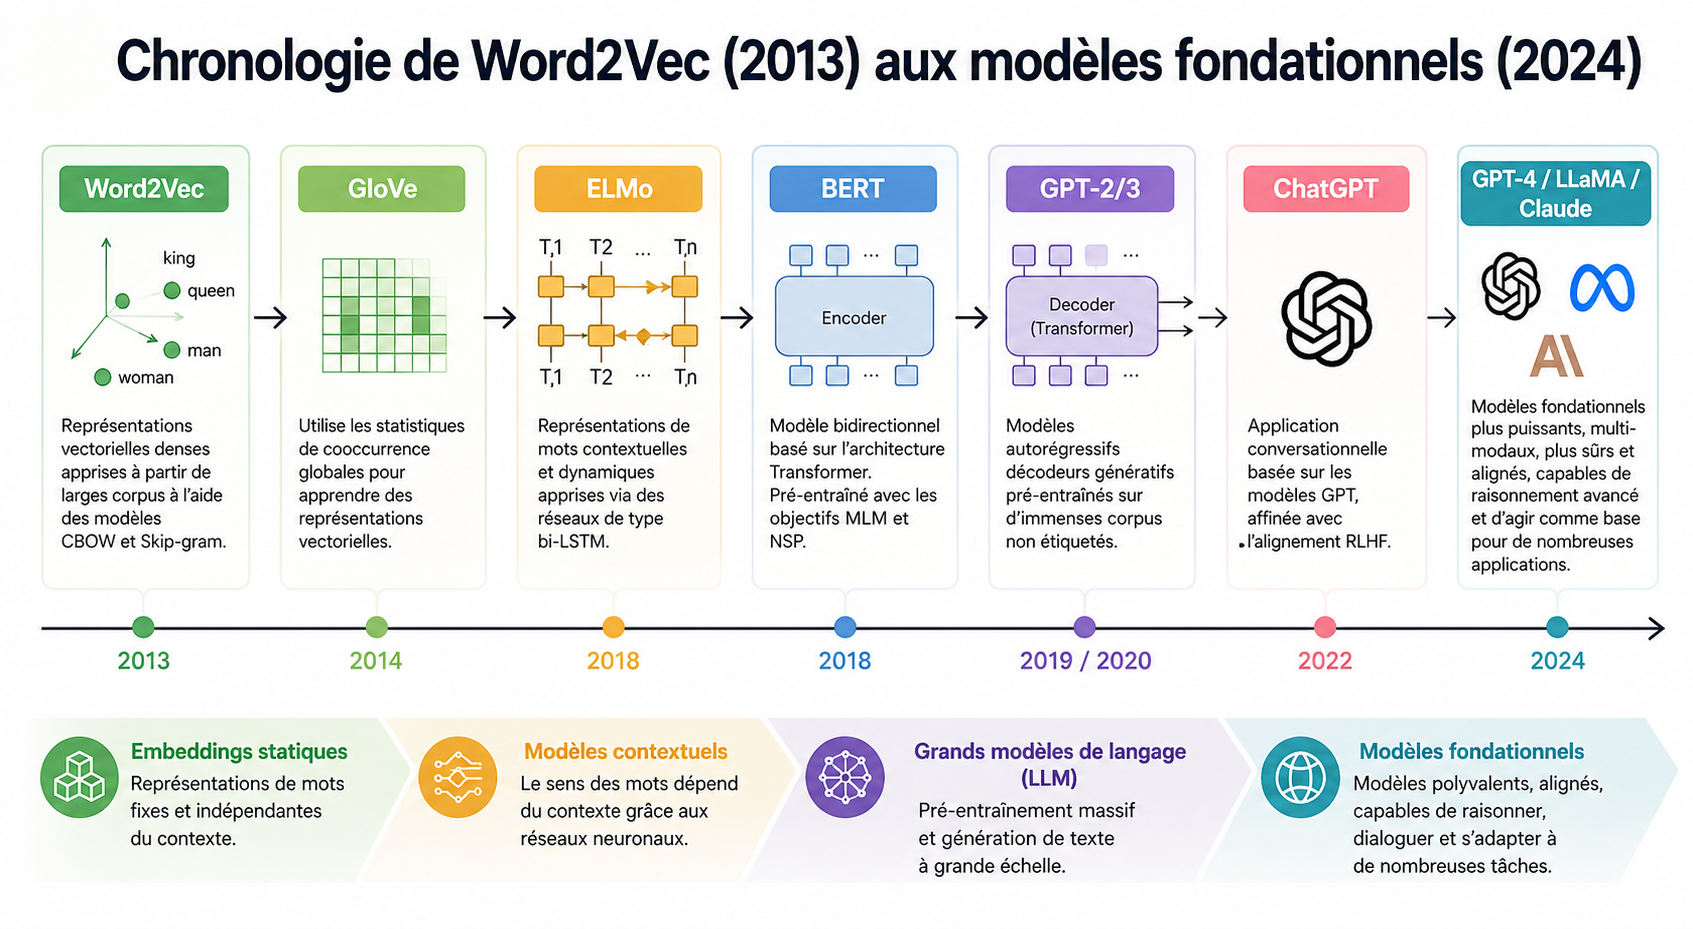
\includegraphics[width=0.75\textwidth]{figures/evolution_llms.png}
  \source{Auteur}
\end{figure}
\subsubsection{Les représentations vectorielles denses Word2Vec (2013):}
L'introduction de Word2Vec par Mikolov et al. (2013) marque une rupture majeure. A l'aide d'un réseau de neurones peu profond, le modèle apprend des plongements vectoriels (embeddings) qui capturent les régularités sémantiques entre mots, en s'appuyant sur l'hypothèse distributionnelle selon laquelle « des mots qui apparaissent dans des contextes similaires ont des sens similaires ». Pour la première fois, des opérations algébriques sur les vecteurs de mots (par exemple roi - homme + femme = reine) deviennent significatives. Word2Vec produit toutefois des représentations statiques : le mot « banque » a la même représentation, qu'il désigne une institution financière ou la rive d'un fleuve.

\subsubsection{Les réseaux récurrents et l'introduction de l'attention (2014-2016)}
Pour modéliser le caractère séquentiel du langage, les RNN, notamment dans leurs variantes LSTM et GRU, ont été largement adoptés. Couplés en architecture encodeur-décodeur, ils ont permis d'aborder des tâches complexes comme la traduction automatique. Cependant, le traitement séquentiel impose la compression de toute l'information d'une phrase d'entrée dans un unique vecteur de contexte, ce qui dégrade les performances sur les longues séquences. Bahdanau, Cho et Bengio (2014) introduisent alors le mécanisme d'attention, qui permet au décodeur de pondérer dynamiquement les états cachés de l'encodeur et de « se concentrer » sur les portions pertinentes de la séquence d'entrée à chaque étape de génération.

\subsubsection{Le Transformer et l'ère des LLMs (2017-aujourd'hui)}
En 2017, Vaswani et al. publient l'article fondateur « Attention Is All You Need », qui propose une architecture entièrement fondée sur l'attention et abandonne la récurrence. L'architecture Transformer se révèle hautement parallélisable, ce qui ouvre la voie à un passage à l'échelle sans précédent. Elle donne naissance, dès 2018, à deux familles de modèles :
\begin{itemize}
    \item \textbf{BERT} (Bidirectional Encoder Representations from Transformers, Devlin et al., 2018), modèle encodeur seul, dédié à la représentation contextuelle du texte ;
    \item \textbf{GPT} (Generative Pre-trained Transformer, Radford et al., 2018), modèle décodeur seul, dédié à la génération de texte.
\end{itemize}
La trajectoire des modèles GPT illustre la dynamique d'échelle qui caractérise l'ère des LLMs : 117 millions de paramètres pour GPT-1 (2018), 1,5 milliard pour GPT-2 (2019), 175 milliards pour GPT-3 (2020). Le lancement public de ChatGPT en novembre 2022, fondé sur GPT-3.5 puis GPT-4, marque la diffusion massive de ces technologies, atteignant 100 millions d'utilisateurs actifs en deux mois. Parallèlement, l'écosystème open source (LLaMA, Mistral, Falcon) et de nouvelles architectures (Mamba, RWKV) viennent enrichir le paysage en proposant des compromis variés entre coût computationnel, longueur de contexte et qualité de génération.

% ────────────────────────────────────────────────────────────
\subsection{Le concept d'embeddings et représentations vectorielles}
% ────────────────────────────────────────────────────────────
Le langage humain est une donnée non structurée que les ordinateurs ne peuvent traiter directement sous sa forme brute. Pour qu'un modèle de langage puisse manipuler et « calculer » le sens, il est indispensable de convertir au préalable le texte en représentations numériques appelées vecteurs. Cette opération de transformation porte le nom d'embedding (plongement vectoriel).Les \textit{embeddings} constituent la représentation numérique fondamentale sur laquelle repose tout le pipeline de matching emploi-compétences. Un embedding est une projection
d'un objet (mot, phrase, document, compétence) dans un espace vectoriel continu de
dimension $d$, typiquement $d \in [128,\; 4096]$, où la proximité géométrique reflète
la similarité sémantique. L'objectif d'un modèle d'embedding est de produire des représentations qui restituent, dans un espace mathématique, le sens des unités linguistiques de la manière la plus précise possible. Autrement dit, l'embedding constitue le pont entre le langage humain discret, symbolique et fortement ambigu et les opérations algébriques que les réseaux de neurones sont en mesure d'effectuer.
\subsubsection{Embeddings statiques vs. contextuels}
\begin{table}[H]
  \centering
  \caption{Comparaison des embeddings statiques et contextuels.}
  \label{tab:embeddings}
  \small
  \begin{tabularx}{\linewidth}{>{\bfseries}lXX}
    \toprule
    \rowcolor{kmeraiteal!90}
    \textcolor{white}{\textbf{Propriété}}
    & \textcolor{white}{\textbf{Statiques (Word2Vec, GloVe)}}
    & \textcolor{white}{\textbf{Contextuels (\BERT{}, GPT)}} \\
    \midrule
    \rowcolor{kmeraiteal!12}
    Dépendance au contexte & Non - un mot $=$ un vecteur unique & Oui - vecteur différent selon le contexte \\
    \rowcolor{kmeraigreen!8}
    Capture de polysémie & Limitée & Excellente \\
    \rowcolor{kmeraiteal!12}
    Exemple & \og Bank\fg{} $=$ même vecteur (banque/rive) & \og Bank\fg{} varie selon la phrase \\
    \rowcolor{kmeraigreen!8}
    Usage en NLP moderne & Rare (benchmarks historiques) & Dominant \\
    \rowcolor{kmeraiteal!12}
    Coût computationnel & Faible & Élevé (GPU requis) \\
    \bottomrule
  \end{tabularx}
  \source{Auteur}
\end{table}

\subsubsection{Le rôle des embeddings dans l'architecture Transformer}
Dans un modèle Transformer, les embeddings constituent la première étape du traitement. Le pipeline d'entrée se déroule selon les étapes suivantes :
\begin{enumerate}
    \item Le texte d'entrée est segmenté en jetons (tokens) par un algorithme de tokenisation, généralement de type sous-mots (Byte-Pair Encoding, WordPiece ou SentencePiece).
    \item Chaque jeton est associé à un vecteur initial issu d'une matrice d'embeddings apprise lors du pré-entraînement et indexée par les identifiants des jetons du vocabulaire.
    \item Un codage positionnel (positional encoding) est ajouté à ces vecteurs afin que le modèle puisse exploiter l'ordre des mots dans la séquence, l'architecture Transformer traitant l'ensemble des jetons simultanément et n'ayant donc, par construction, aucune notion intrinsèque d'ordre.
    \item Les vecteurs ainsi enrichis circulent à travers les couches successives du modèle, où ils sont progressivement contextualisés par les mécanismes d'auto-attention et les réseaux de propagation avant.
\end{enumerate} 
%FIGURE






% ────────────────────────────────────────────────────────────
\subsection{L'architecture Transformer et le mécanisme d'attention}
% ────────────────────────────────────────────────────────────
 
L'architecture Transformer, introduite par \citeauthor{vaswani2017attention} (\citeyear{vaswani2017attention})
dans le célèbre article \textit{Attention Is All You Need}, constitue le paradigme architectural
dominant dans le traitement du langage naturel. Elle repose sur un mécanisme d'auto-attention
(\textit{self-attention}) qui permet au modèle d'examiner simultanément l'ensemble des positions
d'une séquence d'entrée pour calculer des représentations contextualisées de chaque token.
 
\subsubsection{Le mécanisme d'auto-attention}
 
Formellement, étant donnée une séquence de vecteurs d'entrée $\mat{X} \in \R^{n \times d}$,
le mécanisme d'attention produit une sortie en calculant trois matrices : les requêtes $\mat{Q}$,
les clés $\mat{K}$ et les valeurs $\mat{V}$, obtenues par projections linéaires apprises :
 
\begin{equation}
  \mat{Q} = \mat{X}\mat{W}^Q, \quad
  \mat{K} = \mat{X}\mat{W}^K, \quad
  \mat{V} = \mat{X}\mat{W}^V
\end{equation}
 
La sortie de l'attention est alors :
 
\begin{equation}
  \operatorname{Attention}(\mat{Q}, \mat{K}, \mat{V})
  = \softmax\!\left(\frac{\mat{Q}\mat{K}^\top}{\sqrt{d_k}}\right)\mat{V}
  \label{eq:attention}
\end{equation}
 
où $d_k$ est la dimension des vecteurs clés, utilisée pour normaliser le produit scalaire
et éviter des gradients trop faibles. Ce mécanisme permet à chaque token de \og regarder \fg{}
tous les autres tokens de la séquence simultanément, contrairement aux architectures récurrentes
(RNN, LSTM) qui traitent les tokens séquentiellement.
Dans le contexte du matching
emploi-compétences, cela signifie que le modèle peut mettre en relation le terme \og Python \fg{}
d'un CV avec \og développement back-end \fg{} dans une offre d'emploi, même si ces termes
sont distants dans le texte.
\subsubsection{L'attention multi-têtes} L'architecture utilise Afin de capturer simultanément des relations linguistiques de natures variées, le Transformer ne se limite pas à un unique calcul d'attention. Il met en œuvre une attention multi-têtes, c'est-à-dire plusieurs calculs d'attention exécutés en parallèle (typiquement 8 ou 12 têtes, parfois davantage dans les modèles de plus grande taille).Chaque tête d'attention dispose de ses propres matrices de projection $Q$,$K$ et $V$, apprises de manière indépendante comme le montre la \ref{fig:self_attention}. Elle peut ainsi se spécialiser dans l'identification d'un type particulier de relation : dépendances syntaxiques, proximité sémantique, coréférence pronominale, reconnaissance d'entités, etc. Les sorties des différentes têtes sont ensuite concaténées puis projetées linéairement pour produire la représentation finale.Cette architecture confère au modèle une capacité d'expression supérieure et lui permet d'analyser une même séquence sous plusieurs angles complémentaires.
\begin{figure}[H]
  \centering
  \caption{Mécanisme de self-attention}
  \label{fig:self_attention}
  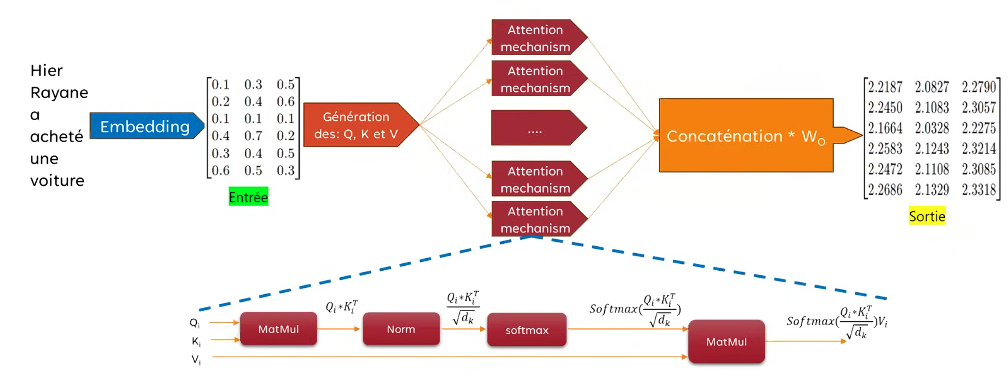
\includegraphics[width=0.8\textwidth]{figures/self_attention.png}
  \source{Auteur}
\end{figure}
%\begin{align}
%  \operatorname{MultiHead}(\mat{Q},\mat{K},\mat{V})
 % &= \operatorname{Concat}(\text{head}_1, \ldots, %\text{head}_h)\,\mat{W}^O \\
%  \text{avec} \quad \text{head}_i
%  &= \operatorname{Attention}(\mat{Q}\mat{W}_i^Q,\; %\mat{K}\mat{W}_i^K,\; \mat{V}\mat{W}_i^V)
 % \label{eq:multihead}
%\end{align}
\subsubsection{Composants internes d'un bloc Transformer}
Au-delà de l'attention, la figure \ref{fig:transformers} montre que chaque bloc Transformer comprend deux éléments complémentaires essentiels au bon fonctionnement de l'architecture :
\begin{itemize}
    \item \textbf{Le réseau de neurones à propagation avant (Feedforward Neural Network, FFN).} Appliqué de manière indépendante à chaque position de la séquence, il constitue la majeure partie de la capacité de traitement et de mémorisation du modèle. C'est dans cette sous-couche qu'est essentiellement stockée la connaissance acquise lors du pré-entraînement.
    \item \textbf{Les connexions résiduelles et la normalisation de couche.} Les connexions résiduelles (residual connections) facilitent la propagation de l'information et du gradient à travers les couches profondes, tandis que les techniques de normalisation Layer Normalization dans la formulation originale, RMSNorm dans les architectures plus récentes stabilisent l'entraînement et accélèrent la convergence.
\end{itemize}
L'enchaînement de ces éléments self-attention, normalisation, FFN, connexions résiduelles est répété un grand nombre de fois (de 12 couches pour les modèles de petite taille à plus d'une centaine pour les plus grands LLMs), ce qui permet au modèle de construire des représentations linguistiques de plus en plus abstraites au fil des couches.
\begin{figure}[H]
  \centering
  \caption{Architecture complète du Transformer}
  \label{fig:transformers}
  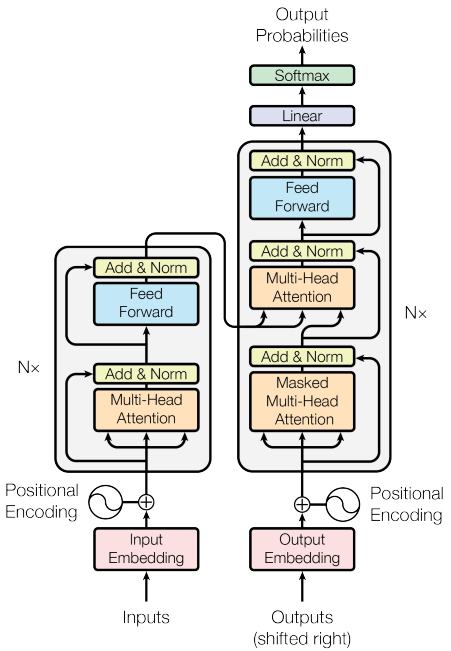
\includegraphics[width=0.5\textwidth]{figures/trans.png}
  \source{Auteur}
\end{figure}
%\subsubsection{Spécificités du décodeur : attention masquée et attention croisée}
%Le décodeur du Transformer présente deux caractéristiques distinctives qui le différencient de l'encodeur.
%\begin{itemize}
 %   \item \textbf{L'auto-attention masquée (Masked Self-Attention).} Dans le décodeur, le mécanisme d'auto-attention est restreint par un masque qui empêche tout jeton de la séquence de sortie de « regarder vers le futur ». Concrètement, lors du calcul des scores d'attention, les positions correspondant à des jetons non encore générés sont annulées (typiquement par affectation d'un score infini avant l'application du softmax). Cette contrainte est indispensable à la cohérence du processus de génération autorégressive : à chaque étape, le modèle ne doit s'appuyer que sur les jetons déjà produits.
 %   \item \textbf{L'attention croisée (Cross-Attention).} Dans l'architecture encodeur-décodeur originale, le décodeur intègre, en plus de son auto-attention masquée, une couche d'attention croisée qui établit le lien avec l'encodeur. Dans cette couche, les vecteurs Requête proviennent de la séquence en cours de génération (côté décodeur), tandis que les vecteurs Clé et Valeur proviennent de la représentation produite par l'encodeur. Ce mécanisme permet au décodeur d'aligner sa production sur les informations contenues dans la séquence d'entrée propriété fondamentale dans les tâches de type séquence-vers-séquence telles que la traduction automatique ou la synthèse de documents.
%\end{itemize}
% ────────────────────────────────────────────────────────────
\subsection{Variantes architecturales des \LLM{}s}
% ────────────────────────────────────────────────────────────
 
Selon leur architecture, les \LLM{}s se distinguent principalement en trois familles,
chacune présentant des avantages spécifiques pour les sous-tâches du système de recommandation.
 
\subsubsection{Modèles à encodeur seul (\textit{Encoder-only})}
 
\BERT{} \cite{devlin2018bert} et ses variantes (RoBERTa, CamemBERT, XLM-R) sont optimisés
pour la compréhension et la classification de texte. Leur mécanisme bidirectionnel leur permet
de traiter le contexte gauche \textbf{et} droit simultanément, ce qui est idéal pour
l'extraction d'entités (compétences, diplômes, expériences) à partir de CV ou d'offres
d'emploi, ainsi que pour la classification de niveau de qualification.
 
\subsubsection{Modèles à décodeur seul (\textit{Decoder-only})}
 
GPT \cite{radford2018gpt}, LLaMA \cite{touvron2023llama} et leurs successeurs sont spécialisés
dans la génération de texte. \citeauthor{muennighoff2022sgpt} (\citeyear{muennighoff2022sgpt})
propose SGPT, qui utilise des modèles GPT comme bi-encodeurs pour la recherche sémantique
asymétrique, produisant des sentence embeddings sémantiquement riches par
\textit{contrastive fine-tuning}.
 
\subsubsection{Modèles encodeur-décodeur (\textit{Seq2Seq})}
 
T5 \cite{raffel2020t5} et BART reformulent toutes les tâches NLP comme des problèmes de
séquence à séquence. Leur flexibilité les rend utiles pour la traduction entre nomenclatures
de compétences différentes (par exemple, entre la \NCM{} camerounaise et le référentiel \ESCO{}).
 
\begin{table}[H]
  \centering
  \caption{Variantes architecturales des \LLM{}s et leurs applications au matching emploi-compétences.}
  \label{tab:llm_variants}
  \small
  \begin{tabularx}{\linewidth}{lllX}
    \toprule
    \rowcolor{kmeraiteal!90}
    \textcolor{white}{\textbf{Architecture}}
    & \textcolor{white}{\textbf{Exemples}}
    & \textcolor{white}{\textbf{Points forts}}
    & \textcolor{white}{\textbf{Application au matching}} \\
    \midrule
    \rowcolor{kmeraiteal!12}
    Encodeur seul & \BERT{}, RoBERTa & Classification, extraction & Extraction de compétences CV/offres \\
    \rowcolor{kmeraigreen!8}
    Décodeur seul & GPT-4, LLaMA & Génération, zero-shot & Enrichissement de profils, recommandations \\
    \rowcolor{kmeraiteal!12}
    Encodeur-Décodeur & T5, BART & Traduction, résumé & Alignement inter-référentiels \\
    \bottomrule
  \end{tabularx}
  \source{Auteur}
\end{table}

\section{Généralité sur le fine-tuning des modèles de \LLM{}s}
Le \emph{fine-tuning}, ou ajustement fin, désigne l'adaptation d'un modèle pré-entraîné à une tâche, un domaine ou un style de réponse spécifique. Dans le cas des \LLM{}s, le modèle dispose déjà de connaissances linguistiques et statistiques acquises lors d'un pré-entraînement massif sur de grands corpus. Le fine-tuning ne repart donc pas de zéro : il modifie une partie ou la totalité des paramètres du modèle afin d'améliorer ses performances sur un corpus plus spécialisé \cite{devlin2018bert,raffel2020t5}. Cette logique est particulièrement pertinente lorsque le domaine cible possède un vocabulaire, des relations sémantiques ou des critères de décision qui diffèrent des usages généraux du langage.

Dans le cadre du matching emploi-compétences, l'intérêt du fine-tuning est direct. Les textes manipulés ne sont pas de simples phrases ordinaires ; ce sont des CV, des offres d'emploi, des intitulés de métiers, des descriptions de tâches, des compétences techniques, des certifications et des parcours de formation. Un modèle généraliste peut comprendre une partie de ces informations, mais il peut confondre des compétences proches, ignorer des synonymes professionnels locaux ou mal hiérarchiser l'importance d'une compétence dans une offre. L'ajustement sur des données du domaine permet de spécialiser les représentations du modèle afin qu'il rapproche mieux les profils et les postes réellement compatibles.

\subsection{Pré-entraînement, adaptation et spécialisation}
Le pré-entraînement consiste à exposer un modèle à de très grands volumes de textes afin qu'il apprenne des régularités générales du langage. Selon l'architecture, l'objectif peut être de prédire des mots masqués, comme dans \BERT{}, ou de prédire le prochain token, comme dans les modèles génératifs de type GPT \cite{devlin2018bert,brown2020language}. Cette phase produit un modèle généraliste, puissant mais non spécialisé.

Le fine-tuning intervient ensuite comme une phase d'adaptation. On fournit au modèle des exemples représentatifs du problème cible : paires CV--offre, couples compétence--métier, descriptions de formation--compétences développées, ou encore triplets du type \textit{offre, compétence requise, niveau attendu}. Le modèle apprend alors à ajuster ses représentations internes aux régularités du domaine. Dans un système emploi-compétences, l'objectif n'est pas seulement de générer du texte ; il est surtout d'améliorer l'extraction d'entités, la classification des compétences, la recherche sémantique et le classement des recommandations.

Il faut néanmoins éviter une erreur fréquente : fine-tuner un \LLM{} ne garantit pas automatiquement un meilleur système. Si les données sont faibles, bruitées ou biaisées, le modèle apprendra ces biais. Si les labels sont incohérents, le fine-tuning dégradera la qualité des représentations. Si le domaine est mal défini, l'adaptation risque d'être superficielle. La qualité du corpus, la définition des tâches et la cohérence des annotations sont donc plus importantes que la seule taille du modèle.

\subsection{Les principales formes de fine-tuning}
On distingue plusieurs formes d'adaptation, selon l'objectif et les ressources disponibles.

\subsubsection{Fine-tuning supervisé}
Le fine-tuning supervisé utilise des données annotées. Dans le cas du matching emploi-compétences, il peut s'agir de paires \textit{profil--offre} annotées comme pertinentes ou non pertinentes, de compétences extraites manuellement de CV, ou de descriptions associées à une catégorie métier. Le modèle apprend à reproduire ces décisions. Cette approche est utile pour des tâches comme la classification, l'extraction d'entités et le scoring de similarité.

\subsubsection{Instruction tuning}
L'\emph{instruction tuning} adapte le modèle à suivre des consignes formulées en langage naturel. Au lieu de seulement prédire une classe ou une similarité, le modèle apprend à répondre à des demandes telles que : \og extrais les compétences techniques de ce CV \fg{}, \og identifie les compétences manquantes pour cette offre \fg{} ou \og propose une formation pour combler cet écart \fg{}. Les travaux d'Ouyang et al. montrent que l'ajustement sur des instructions et préférences humaines améliore l'utilité perçue des réponses des grands modèles de langage \cite{ouyang2022training}.

\subsubsection{Fine-tuning contrastif pour les embeddings}
Pour la recherche sémantique, le fine-tuning peut viser non pas la génération de texte, mais la qualité des embeddings. L'objectif est alors de rapprocher dans l'espace vectoriel les éléments similaires et d'éloigner les éléments non similaires. Par exemple, une offre de \og data analyst \fg{} et un profil maîtrisant Python, SQL, Excel, visualisation et statistiques doivent être proches ; une offre de comptabilité pure et un profil de développement web doivent être plus éloignés. Cette logique de fine-tuning contrastif est centrale pour les modèles de type Sentence-BERT \cite{reimers2019sbert}.

\subsubsection{Adaptation légère des paramètres}
Le fine-tuning complet d'un \LLM{} peut être coûteux, car il met à jour tous les paramètres du modèle. Les méthodes d'adaptation efficace, comme LoRA, réduisent ce coût en insérant de petites matrices entraînables dans certaines couches du réseau, tout en gardant la majorité des paramètres gelés \cite{hu2021lora}. QLoRA pousse cette logique plus loin en combinant quantification et adaptation légère, ce qui permet d'ajuster de grands modèles avec beaucoup moins de mémoire GPU \cite{dettmers2023qlora}. Pour un projet appliqué comme celui-ci, ces méthodes sont souvent plus réalistes qu'un fine-tuning complet.

\subsection{Application au matching emploi-compétences}
Dans le système proposé, le fine-tuning peut intervenir à trois niveaux complémentaires. Le premier niveau concerne l'extraction : le modèle doit identifier dans les textes les compétences, outils, diplômes, années d'expérience, secteurs et métiers. Le deuxième niveau concerne la représentation : les embeddings doivent capturer les similarités professionnelles, y compris lorsque les formulations sont différentes. Le troisième niveau concerne l'explication : le modèle doit être capable de produire une justification lisible, par exemple en distinguant les compétences acquises, les compétences manquantes et les formations recommandées.

Cette architecture suppose une articulation rigoureuse avec la nomenclature métiers-compétences. Le fine-tuning ne doit pas seulement apprendre des régularités textuelles ; il doit être contraint par un référentiel. Par exemple, si le modèle extrait \og Power BI \fg{}, \og tableau de bord \fg{} et \og reporting \fg{}, ces éléments doivent pouvoir être rattachés à une compétence standardisée de visualisation ou d'aide à la décision. C'est cette normalisation qui permet ensuite d'alimenter correctement le graphe de connaissances.

\subsection{Risques et précautions méthodologiques}
Le fine-tuning présente plusieurs risques. Le premier est le sur-apprentissage : le modèle peut mémoriser les exemples du corpus sans généraliser à de nouvelles offres. Le deuxième est le biais de données : si les offres collectées favorisent certains secteurs, niveaux de diplôme ou formulations linguistiques, le modèle reproduira ces déséquilibres. Le troisième est la perte de robustesse : un modèle trop spécialisé peut devenir moins performant sur des formulations inattendues. Enfin, le quatrième risque est l'opacité : si le modèle produit un score sans explication, il sera difficile de convaincre un utilisateur ou un recruteur de la pertinence de la recommandation.

Ces limites justifient le recours à un système hybride. Le \LLM{} apporte la compréhension linguistique ; la base vectorielle apporte la recherche par similarité ; le graphe de connaissances apporte la structure, les contraintes et l'explicabilité. Dans cette perspective, le fine-tuning n'est pas une fin en soi. Il est un levier d'adaptation qui doit rester subordonné à l'objectif central du mémoire : produire un matching emploi-compétences plus pertinent, plus interprétable et plus utile pour la montée en compétences.


% ============================================================
\section{Généralité sur des BD vectorielles et orientées graphes}
% ============================================================
Les bases de données vectorielles et les bases orientées graphes répondent à deux besoins complémentaires dans les systèmes modernes d'intelligence artificielle. Les premières sont conçues pour indexer et interroger des représentations numériques continues, généralement produites par des modèles d'embeddings. Les secondes sont conçues pour représenter explicitement des entités et les relations qui les relient. Dans le cadre du matching emploi-compétences, cette complémentarité est stratégique : la base vectorielle permet de retrouver des profils et offres proches sur le plan sémantique, tandis que le graphe permet d'expliquer pourquoi ces éléments sont liés à travers des métiers, compétences, secteurs, formations et niveaux d'exigence.

\subsection{Structure générale d'une base de données vectorielle}
Une base de données vectorielle est un système de stockage et de recherche optimisé pour des vecteurs numériques de grande dimension. Chaque objet textuel, par exemple un CV, une offre d'emploi, une compétence ou une description de formation, est transformé en embedding par un modèle de représentation. Cet embedding est ensuite stocké avec un identifiant, des métadonnées et parfois le texte source. La base ne manipule donc pas seulement des chaînes de caractères ; elle manipule des points dans un espace vectoriel où la distance ou la proximité traduit une forme de similarité sémantique.

La structure minimale d'une base vectorielle comprend généralement quatre composantes. La première est le \textit{document source}, c'est-à-dire l'information initiale : CV, offre, compétence, métier ou contenu de formation. La deuxième est le \textit{vecteur d'embedding}, qui encode ce document dans un espace numérique. La troisième est l'ensemble des \textit{métadonnées}, comme le pays, le secteur, le niveau d'expérience, la date de collecte ou le type d'objet. La quatrième est l'\textit{index vectoriel}, qui accélère la recherche des plus proches voisins.

Dans un système de matching emploi-compétences, une table vectorielle peut par exemple contenir les colonnes suivantes : un identifiant d'offre, le texte nettoyé de l'offre, le vecteur associé, le secteur d'activité, le niveau d'expérience requis et la liste normalisée des compétences extraites. Une requête utilisateur, comme un profil candidat, est vectorisée à son tour. Le système compare ensuite ce vecteur avec ceux de la base afin d'identifier les offres les plus proches.

La difficulté principale vient du fait que les embeddings sont souvent de grande dimension. Une recherche exhaustive sur tous les vecteurs devient coûteuse lorsque la base contient des milliers ou millions d'objets. C'est pourquoi les bases vectorielles utilisent des index de recherche approximative des plus proches voisins, tels que HNSW ou IVF, largement employés dans les moteurs spécialisés comme FAISS ou dans des extensions comme pgvector \cite{malkov2018hnsw,johnson2019faiss,pgvector2024}.

\subsection{Principe de la recherche sémantique dans une BD vectorielle}
La recherche sémantique consiste à retrouver des objets proches par le sens plutôt que par la présence exacte des mêmes mots. Contrairement à une recherche lexicale classique, qui dépend fortement des mots-clés, elle exploite la position des embeddings dans un espace vectoriel. Deux textes peuvent donc être rapprochés même s'ils n'emploient pas les mêmes termes. Par exemple, une offre mentionnant \og conception de tableaux de bord décisionnels \fg{} peut être rapprochée d'un profil indiquant \og Power BI, reporting et visualisation de données \fg{}.

Le processus comprend généralement cinq étapes. Premièrement, les textes sont nettoyés et segmentés. Deuxièmement, un modèle d'embedding transforme chaque texte en vecteur. Troisièmement, les vecteurs sont stockés et indexés. Quatrièmement, la requête est elle-même transformée en vecteur. Cinquièmement, la base retourne les objets les plus proches selon une mesure de similarité.

Les mesures les plus utilisées sont la similarité cosinus, la distance euclidienne et le produit scalaire. La similarité cosinus est particulièrement fréquente en traitement du langage, car elle mesure l'angle entre deux vecteurs et neutralise en partie l'effet de leur norme. Elle est définie par :

\begin{equation}
\cos(\vec{u}, \vec{v}) =
\frac{\vec{u}\cdot\vec{v}}{\|\vec{u}\|\|\vec{v}\|}
\end{equation}

Dans le cas du matching emploi-compétences, cette recherche permet de produire une première liste d'offres candidates pour un profil donné. Toutefois, un score vectoriel seul ne suffit pas. Il peut identifier une proximité globale, mais il ne dit pas toujours quelles compétences expliquent cette proximité, quelles compétences manquent, ni quelle formation pourrait combler l'écart. C'est précisément la limite qui justifie l'association avec une base orientée graphe.

\subsection{Structure générale d'une base de données orientée graph}
Une base de données orientée graphe représente l'information sous forme de nœuds et de relations. Les nœuds désignent les entités du domaine, tandis que les relations décrivent les liens entre ces entités. Cette logique diffère des bases relationnelles classiques, où les relations sont généralement reconstituées par des jointures entre tables. Dans une base graphe, les liens sont des objets de première classe : ils sont stockés, typés, parcourus et analysés directement.

Dans le domaine emploi-compétences, les nœuds peuvent représenter des candidats, offres, métiers, compétences, secteurs, formations, certifications ou niveaux de qualification. Les relations peuvent exprimer des liens tels que \textit{possède}, \textit{exige}, \textit{appartient à}, \textit{développe}, \textit{est similaire à} ou \textit{prépare à}. Cette représentation est beaucoup plus proche de la structure réelle du marché de l'emploi, car un métier n'est pas une simple ligne de table : il est défini par un ensemble de compétences, d'activités, de niveaux, de secteurs et de trajectoires possibles.

Formellement, un graphe peut être défini comme un couple $G=(V,E)$, où $V$ désigne l'ensemble des nœuds et $E$ l'ensemble des relations. Dans un graphe de connaissances, les relations sont souvent représentées sous forme de triplets :

\begin{equation}
(\text{sujet},\ \text{relation},\ \text{objet})
\end{equation}

Par exemple, le triplet $(\text{Data Analyst},\ \text{exige},\ \text{SQL})$ signifie que la compétence SQL est requise pour le métier de data analyst. De même, $(\text{Formation Power BI},\ \text{développe},\ \text{Visualisation de données})$ indique qu'une formation contribue à développer une compétence standardisée.

Les bases graphes comme Neo4j permettent ensuite d'interroger ces relations avec des langages adaptés, notamment Cypher. Un système peut ainsi répondre à des questions que la recherche vectorielle seule gère mal : quelles compétences manquent à un candidat pour viser un métier ? Quelles formations développent ces compétences ? Quelles offres sont proches d'un profil si l'on accepte une trajectoire de formation courte ?
  
\subsection{Techniques de description et d'analyse des graphes de connaissances}
Un graphe de connaissances ne sert pas seulement à stocker des relations ; il permet aussi de les analyser. Les techniques de description de graphe visent à comprendre la structure du réseau, l'importance relative des entités et les chemins qui relient les objets. Dans un système emploi-compétences, ces analyses peuvent aider à identifier les compétences centrales, les métiers passerelles, les formations les plus utiles ou les trajectoires de reconversion les plus plausibles.

Une première famille de techniques concerne les mesures de centralité. La centralité de degré mesure le nombre de connexions directes d'un nœud. Une compétence fortement connectée à de nombreux métiers, comme Excel, SQL ou communication professionnelle, peut être considérée comme transversale. La centralité d'intermédiarité mesure la fréquence avec laquelle un nœud se trouve sur les chemins les plus courts entre d'autres nœuds ; elle permet d'identifier des compétences ou formations jouant un rôle de passerelle entre plusieurs familles de métiers. La centralité de proximité mesure la distance moyenne d'un nœud à tous les autres, indiquant sa capacité à atteindre rapidement le reste du réseau.

Une deuxième famille concerne la recherche de chemins. Dans le matching emploi-compétences, les chemins permettent de produire des recommandations explicables. Si un candidat possède Python et statistiques, et qu'une offre exige aussi SQL et Power BI, le graphe peut identifier les compétences manquantes, puis rechercher les formations qui les développent. L'explication ne repose donc pas uniquement sur un score opaque ; elle repose sur un chemin interprétable entre profil, compétences, offre et formation.

Une troisième famille concerne la détection de communautés. Elle permet de repérer des groupes de métiers ou de compétences fortement liés entre eux. Par exemple, les métiers de la data peuvent former une communauté autour des compétences Python, SQL, statistiques, visualisation et machine learning, tandis que les métiers du marketing numérique peuvent former une autre communauté autour du SEO, de la publicité en ligne, de l'analyse d'audience et de la stratégie de contenu. Ces regroupements peuvent aider à structurer les parcours de formation et les recommandations de reconversion.

Enfin, les graphes de connaissances peuvent être enrichis par des représentations vectorielles de graphes, ou \textit{graph embeddings}. Ces méthodes projettent les nœuds et relations dans un espace vectoriel afin de faciliter la prédiction de liens, la classification de nœuds ou la recommandation. Des approches plus avancées, comme les réseaux de neurones sur graphes, exploitent la structure locale du graphe pour apprendre des représentations tenant compte du voisinage des entités \cite{hogan2021knowledge,hamilton2020graph}.

 
% ────────────────────────────────────────────────────────────
\subsection{Synergie \LLM{} + Graphes de Connaissances}
% ────────────────────────────────────────────────────────────
La combinaison entre \LLM{}s et graphes de connaissances répond à une faiblesse de chacun des deux outils pris isolément. Les \LLM{}s sont puissants pour comprendre et générer du langage naturel, extraire des entités et reformuler des contenus. Cependant, ils peuvent produire des réponses approximatives, manquer de traçabilité ou halluciner des relations non vérifiées. Les graphes de connaissances, à l'inverse, offrent une structure explicite, contrôlable et interrogeable, mais ils nécessitent une alimentation régulière et une normalisation rigoureuse des données.

Dans un pipeline emploi-compétences, les \LLM{}s peuvent intervenir en amont pour extraire automatiquement les entités présentes dans les CV et offres d'emploi : métiers, compétences, diplômes, outils, années d'expérience, secteurs et certifications. Ces entités sont ensuite alignées sur une nomenclature standardisée, comme la \NCM{} ou \ESCO{}, puis insérées dans le graphe sous forme de nœuds et relations. Le graphe sert alors de mémoire structurée du système.

La synergie apparaît aussi au moment de la recommandation. Une base vectorielle peut identifier les offres les plus proches d'un profil, mais le graphe permet de vérifier la cohérence métier de cette proximité. Par exemple, si deux offres sont proches vectoriellement mais appartiennent à des familles de métiers différentes, le graphe peut aider à distinguer une proximité linguistique superficielle d'une proximité professionnelle réelle. Inversement, le graphe peut révéler des correspondances indirectes que la recherche vectorielle ne voit pas, comme une compétence transférable entre deux métiers voisins.

Enfin, cette combinaison améliore l'explicabilité. Un \LLM{} peut générer une recommandation lisible en langage naturel, mais cette recommandation doit être fondée sur des relations vérifiables dans le graphe : compétences possédées, compétences exigées, compétences manquantes, formations associées et trajectoire possible. Le rôle du \LLM{} n'est donc pas d'inventer l'explication ; il est de verbaliser une chaîne de raisonnement structurée par le graphe. Cette logique rejoint les approches de RAG et de GraphRAG, qui cherchent à combiner récupération d'information, génération et structure relationnelle pour produire des réponses plus contextualisées et plus contrôlables \cite{lewis2020rag,hogan2021knowledge}.
 

%%FIGURE


% ============================================================
\section{Généralité sur les systèmes de recommandation}
% ============================================================
Les systèmes de recommandation (\textsc{sr}) sont des outils algorithmiques conçus pour prédire
et suggérer des éléments pertinents à un utilisateur, en se basant sur des informations le
concernant ainsi que sur les caractéristiques des éléments disponibles. Appliqués au marché de
l'emploi, ils permettent de mettre en relation candidats et offres de manière automatisée,
personnalisée et à grande échelle.
Dans un système classique de recommandation, on distingue généralement trois types d'entités : les utilisateurs, les items et les interactions. Dans le commerce électronique, l'utilisateur est un client et l'item est un produit. Dans le cas du présent mémoire, l'utilisateur peut être un candidat ou un membre de la communauté KmerAI, tandis que l'item peut être une offre d'emploi, un métier cible, une compétence ou une formation. Les interactions peuvent correspondre à des candidatures, clics, sauvegardes d'offres, évaluations, historiques de formation ou correspondances validées par un expert.

La recommandation appliquée à l'emploi présente cependant une difficulté plus forte que la recommandation de produits. Une mauvaise recommandation de film a un coût faible ; une mauvaise recommandation professionnelle peut orienter un candidat vers une trajectoire peu adaptée. Le système doit donc prendre en compte la pertinence, mais aussi l'explicabilité, l'équité, le niveau réel du candidat et la faisabilité de la montée en compétences.

\subsection{Filtrage basé sur le contenu (\textit{Content-Based Filtering})}
Le filtrage basé sur le contenu recommande des items similaires à ceux qui correspondent déjà au profil ou aux préférences de l'utilisateur. Il repose sur les caractéristiques des objets. Dans le cas du matching emploi-compétences, ces caractéristiques peuvent être les compétences exigées, le secteur, le niveau d'expérience, le type de contrat, le lieu, le domaine de formation ou les outils techniques demandés.

Son principe est simple : si un candidat possède Python, SQL, statistiques et visualisation de données, le système recherchera des offres contenant des caractéristiques proches, par exemple analyste de données, chargé d'études statistiques ou business intelligence analyst. Les embeddings permettent d'améliorer cette approche en dépassant les mots-clés exacts. Le système peut alors rapprocher \og reporting décisionnel \fg{} de \og tableau de bord \fg{} ou \og visualisation de données \fg{}.

L'avantage principal du filtrage basé sur le contenu est son interprétabilité relative : on peut expliquer une recommandation par les caractéristiques communes entre le profil et l'offre. Sa limite est qu'il tend à enfermer l'utilisateur dans ce qu'il possède déjà. Si un candidat a un profil statistique, le système peut négliger des trajectoires proches mais exigeant une courte montée en compétences vers la data engineering ou le marketing analytics. Cette limite justifie l'introduction du skill gap et des relations de proximité dans le graphe \cite{pazzani2007content}.

\subsection{Des méthodes traditionnelles aux modèles séquentiels et neuronaux}
La revue récente de Redjdal sur les modèles de langage appliqués à la recommandation basée sur les sessions fournit une grille de lecture utile pour situer l'évolution des systèmes de recommandation \cite{redjdal2024sbr}. Même si son terrain porte sur la prédiction du prochain item dans des sessions d'interaction, la logique générale est transposable au matching emploi-compétences : les méthodes traditionnelles sont efficaces lorsque les signaux sont simples, stables et bien observés, mais elles deviennent limitées dès que la décision dépend d'une séquence, d'un contexte, d'une représentation sémantique ou de relations complexes entre entités.

Les approches classiques peuvent être regroupées en trois familles. Les méthodes par règles et mots-clés rapprochent des profils et des offres à partir de termes communs. Elles sont simples à expliquer, mais elles échouent lorsque les mêmes compétences sont décrites avec des formulations différentes. Les méthodes collaboratives exploitent les comportements passés des utilisateurs ou des candidats : consultation, candidature, validation, recrutement ou suivi de formation. Elles peuvent capter des régularités collectives, mais elles exigent un historique fiable et souffrent fortement du démarrage à froid \cite{koren2009matrix}. Les méthodes séquentielles, enfin, modélisent l'ordre des interactions afin de prédire l'action suivante ; elles sont centrales dans la recommandation basée sur les sessions, comme le montrent les travaux sur les RNN et les mécanismes d'attention \cite{hidasi2015session,li2017narm}.

Dans le cas du marché de l'emploi camerounais, ces trois familles ne suffisent pas prises isolément. Les données d'interaction candidat--offre sont souvent rares ou incomplètes ; les intitulés de postes sont hétérogènes ; les compétences peuvent être implicites dans les descriptions ; et la décision ne dépend pas uniquement de la préférence du candidat, mais aussi de la faisabilité professionnelle. Une offre pertinente doit être proche du profil, compatible avec le niveau de formation, cohérente avec le secteur visé et accessible après une montée en compétences raisonnable. Le problème n'est donc pas seulement de prédire un clic ou une candidature ; il est de produire une recommandation défendable pour un recruteur, un conseiller d'orientation ou un candidat.

\subsection{Apports des graphes et des GNN dans la recommandation}
Une contribution importante de la littérature récente est d'avoir montré l'intérêt des structures de graphe pour représenter les relations entre utilisateurs, items et contextes. Redjdal rappelle que les approches à base de graphes se sont imposées dans la recommandation séquentielle parce qu'elles capturent mieux les transitions et les dépendances complexes entre items que les modèles purement linéaires \cite{redjdal2024sbr}. Les travaux sur les graph neural networks et les modèles de recommandation fondés sur les graphes montrent ainsi que la performance ne vient pas seulement de la représentation individuelle des objets, mais aussi de l'information portée par leurs relations \cite{velickovic2018gat,he2020lightgcn}.

Cette idée est directement pertinente pour l'emploi. Un candidat, une offre, un métier, une compétence, une formation et un secteur ne sont pas des objets indépendants. Ils forment un système relationnel : une offre exige des compétences, un candidat possède ou développe certaines compétences, une formation prépare à un domaine, un niveau \NCF{} contraint l'accès à un poste, et un groupe \MEPC{} situe le métier dans une nomenclature nationale. Un graphe de connaissances permet donc de représenter explicitement ces liens au lieu de les laisser implicites dans des vecteurs ou des textes.

La différence entre un graphe de connaissances et un GNN doit cependant être clarifiée. Le présent mémoire ne prétend pas entraîner un GNN complet sur les relations emploi-compétences. Il mobilise d'abord le graphe comme structure explicative et interrogeable : Neo4j sert à vérifier des contraintes, à calculer des écarts de compétences et à tracer les chemins justifiant une recommandation. Cette position est plus prudente et plus défendable dans un contexte où le volume d'interactions validées reste limité. Les GNN constituent une extension possible lorsque les données relationnelles et les labels de validation seront suffisamment nombreux.

\subsection{Transformers et modèles de langage pour la recommandation}
L'autre apport central mis en évidence par Redjdal est le rapprochement entre la recommandation séquentielle et les modèles de langage Transformer. La prédiction du prochain item dans une session peut être rapprochée de la prédiction du prochain token en NLP : dans les deux cas, le modèle apprend à exploiter un contexte pour anticiper l'élément suivant \cite{kang2018sasrec,moreira2021transformers4rec,redjdal2024sbr}. Cette analogie explique l'intérêt croissant pour BERT, GPT, DeBERTa et les architectures de type Transformer dans les systèmes de recommandation.

Pour le présent mémoire, l'enjeu n'est pas de prédire le prochain clic dans une session, mais de représenter correctement des textes d'offres et de profils. Le rôle des Transformers est donc différent : ils servent principalement à construire des embeddings sémantiques. Un encodeur comme Sentence-BERT transforme une phrase, une annonce ou un profil en vecteur dense, ce qui permet de mesurer la proximité de sens entre deux descriptions \cite{reimers2019sbert}. Cette approche est plus adaptée qu'un simple sac de mots lorsque les annonces contiennent des formulations variables, des synonymes, des termes français et anglais, ou des compétences formulées de manière indirecte.

La logique de fine-tuning utilisée dans ce projet s'inscrit dans cette continuité. Le modèle n'est pas entraîné à générer du texte ; il est adapté pour mieux rapprocher deux vues d'une même offre : une vue structurée, issue des métadonnées, et une vue textuelle, issue des compétences et détails de l'annonce. Cette formulation transforme le problème en tâche de recherche sémantique. Elle est cohérente avec la littérature sur les représentations de phrases, mais elle appelle une limite importante : un bon score vectoriel ne prouve pas une compatibilité professionnelle. Il ne dit pas encore si le niveau \NCF{} est suffisant, si les compétences essentielles sont acquises, ni si la trajectoire de formation est réaliste.

\subsection{Vers une recommandation hybride orientée recrutement et montée en compétences}
La synthèse de la littérature conduit à une conclusion méthodologique forte : dans un système emploi-compétences, aucune famille de méthodes ne suffit seule. Le contenu textuel apporte la proximité sémantique ; les référentiels apportent la standardisation ; le graphe apporte la structure relationnelle ; les éventuels signaux collaboratifs apportent l'expérience d'usage lorsqu'ils existent ; et le module génératif apporte une explication en langage naturel. L'hybridation n'est donc pas un choix esthétique, mais une nécessité imposée par la nature du problème \cite{burke2002hybrid,ricci2011recommender}.

Cette hybridation doit toutefois être disciplinée. Un score collaboratif ne doit pas être affirmé si l'historique d'interactions est insuffisant. Un modèle Transformer ne doit pas être présenté comme une preuve de compatibilité métier. Un graphe incomplet ne doit pas être interprété comme une vérité exhaustive sur les compétences. La recommandation robuste doit séparer les signaux : similarité sémantique, couverture des compétences, niveau de formation, cohérence sectorielle et possibilités de montée en compétences. C'est cette séparation qui permet de produire un verdict opérationnel : profil prêt à postuler, profil à recommander avec plan de formation, profil à conserver en vivier ou profil actuellement hors cible.

Ainsi, la revue de littérature oriente directement l'architecture retenue dans ce mémoire. Comme chez Redjdal, les Transformers sont mobilisés parce qu'ils apprennent des représentations riches utiles à la recommandation. Comme dans les approches à base de graphes, les relations entre objets sont indispensables pour dépasser une simple proximité vectorielle. Mais l'application au marché de l'emploi impose une contrainte supplémentaire : la recommandation doit être explicable, prudente et orientée vers la montée en compétences. Le système proposé articule donc recherche sémantique, graphe de connaissances et logique de skill gap afin de recommander non seulement une offre, mais aussi une trajectoire d'amélioration professionnelle.


%\subsection{Filtrage collaboratif (\textit{Collaborative Filtering})}
%Le filtrage collaboratif recommande des items à partir des comportements collectifs observés. L'idée centrale est que deux utilisateurs ayant eu des comportements similaires dans le passé peuvent être intéressés par des items similaires dans le futur. Dans une plateforme d'emploi, cela peut signifier que des candidats ayant des profils et parcours comparables postulent aux mêmes offres, consultent les mêmes formations ou réussissent dans des métiers proches.

%Les méthodes collaboratives peuvent être fondées sur la similarité entre utilisateurs, sur la similarité entre items ou sur des modèles factoriels. Les approches de factorisation matricielle, popularisées notamment dans les systèmes de recommandation à grande échelle, apprennent des représentations latentes des utilisateurs et des items à partir d'une matrice d'interactions \cite{koren2009matrix}. Dans le cas emploi-compétences, cette matrice peut contenir des signaux comme \textit{a consulté}, \textit{a postulé}, \textit{a été retenu}, \textit{a suivi la formation} ou \textit{a validé la compétence}.

%L'avantage du filtrage collaboratif est qu'il capte des régularités que les caractéristiques explicites ne révèlent pas toujours. Sa limite est le problème du démarrage à froid : lorsqu'un nouveau candidat ou une nouvelle offre apparaît sans historique d'interaction, le système dispose de peu d'information comportementale. En contexte camerounais, où les données d'interaction peuvent être rares ou peu structurées, cette limite est importante. Il serait donc imprudent de fonder tout le système uniquement sur du collaboratif.


%\subsection{Filtrage hybride (\textit{Hybrid Filtering})}
%Le filtrage hybride combine plusieurs sources de signal afin de réduire les limites propres à chaque approche. Dans ce mémoire, l'hybridation est particulièrement adaptée, car le problème ne consiste pas seulement à prédire une préférence ; il consiste à évaluer une compatibilité professionnelle, mesurer un écart de compétences et proposer une trajectoire d'amélioration.

%Un moteur hybride emploi-compétences peut combiner quatre scores. Le premier est un score sémantique, issu de la proximité vectorielle entre le profil et l'offre. Le deuxième est un score structurel, issu du graphe de connaissances et des relations entre métiers, compétences et formations. Le troisième est un score collaboratif, issu des comportements observés sur la plateforme. Le quatrième est un score de skill gap, qui pénalise les offres pour lesquelles les compétences manquantes sont trop nombreuses ou trop critiques.

%Une formulation simple du score hybride peut être donnée par :

%\begin{equation}
%Score_{hyb} =
%\alpha S_{sem} + \beta S_{graph} + \gamma S_{collab} - \delta Gap
%\end{equation}

%où $S_{sem}$ désigne la similarité sémantique, $S_{graph}$ la proximité structurelle dans le graphe, $S_{collab}$ le signal collaboratif, $Gap$ l'écart de compétences, et $\alpha$, $\beta$, $\gamma$, $\delta$ des poids à calibrer empiriquement.

%L'intérêt d'une telle architecture est double. D'abord, elle améliore la robustesse du système : si les interactions collaboratives sont faibles, le contenu et le graphe restent exploitables ; si les descriptions textuelles sont ambiguës, le graphe fournit une structure de contrôle. Ensuite, elle améliore l'explicabilité : le système peut indiquer qu'une offre est recommandée parce que le profil est sémantiquement proche, que plusieurs compétences clés sont déjà acquises, que le métier appartient à une trajectoire proche, et que deux formations permettent de combler les compétences manquantes.

%La recommandation hybride est donc cohérente avec l'objectif général du mémoire. Elle permet de dépasser une logique naïve de mots-clés pour construire un système capable de raisonner sur les compétences, les relations entre métiers et les parcours de montée en qualification \cite{burke2002hybrid,ricci2011recommender}.



% ============================================================
\section{Recherche sémantique et Génération Augmentée par Récupération (\RAG{}) et GraphRAG}
% ============================================================

La recherche sémantique consiste à représenter une requête et un ensemble de documents dans un même espace vectoriel, puis à classer les documents selon leur proximité avec la requête. Contrairement à une recherche par mots-clés, elle ne dépend pas uniquement de la présence des mêmes termes. Elle cherche plutôt à capturer la proximité de sens entre deux formulations. Dans le cadre de ce mémoire, cette propriété est essentielle : un profil mentionnant \og analyse statistique, tableaux de bord et SQL \fg{} doit pouvoir être rapproché d'une offre de \og data analyst \fg{}, même lorsque les formulations exactes ne se recouvrent pas.

La \RAG{} prolonge cette logique en combinant deux opérations : une étape de récupération d'information et une étape de génération. Le système commence par rechercher des passages, documents ou objets structurés pertinents dans une base externe ; il transmet ensuite ces éléments à un modèle génératif, qui produit une réponse conditionnée par le contexte récupéré \cite{lewis2020rag}. Son fonctionnement peut être décomposé en cinq étapes. Premièrement, les documents sont préparés, découpés si nécessaire, puis encodés sous forme de vecteurs. Deuxièmement, ces vecteurs sont stockés dans un index ou une base vectorielle. Troisièmement, lorsqu'une requête arrive, elle est encodée dans le même espace vectoriel que les documents. Quatrièmement, le système récupère les éléments les plus proches selon une mesure comme la similarité cosinus. Cinquièmement, ces éléments sont ajoutés au prompt du modèle génératif afin qu'il produise une réponse fondée sur le contexte récupéré.

Dans cette architecture, le modèle de langage ne répond donc pas seulement à partir de ses connaissances internes. Il reçoit un contexte externe, généralement plus récent, plus spécifique ou plus local que ce qu'il a appris pendant son entraînement. L'intérêt est double. D'une part, le modèle génératif n'est plus obligé de s'appuyer uniquement sur ses paramètres internes, qui peuvent être incomplets ou obsolètes. D'autre part, la réponse peut être rattachée à des sources ou à des éléments vérifiables. Cette architecture reste toutefois fragile lorsque la récupération initiale est mauvaise : si le contexte fourni au modèle est incomplet, bruité ou mal classé, la génération finale peut devenir convaincante en surface mais faible sur le fond.

Dans un système de recommandation emploi-compétences, une \RAG{} purement vectorielle permettrait par exemple de récupérer les offres les plus proches du profil d'un candidat, puis de générer une explication en langage naturel. Cette solution améliore la lisibilité de la recommandation, mais elle reste insuffisante pour juger la compatibilité professionnelle. Deux profils peuvent être proches sémantiquement tout en étant séparés par un niveau de qualification, une contrainte de localisation, une compétence obligatoire ou un domaine de formation. Une offre peut aussi ressembler lexicalement à un profil sans être réellement accessible au candidat.

Le GraphRAG répond à cette limite en introduisant un graphe de connaissances dans la boucle de récupération. Au lieu de transmettre seulement des textes proches, le système récupère également des relations explicites : un candidat possède certaines compétences, une offre en exige d'autres, un métier est associé à des compétences, une formation prépare à un métier, un niveau \NCF{} contraint l'accès à certaines offres, et un groupe \MEPC{} situe le métier dans une nomenclature nationale. Le mécanisme change donc la nature du contexte : la récupération ne porte plus seulement sur des documents similaires, mais aussi sur des chemins de graphe, des voisins, des contraintes et des relations typées. Le graphe permet ainsi de passer d'une proximité textuelle à une explication relationnelle. Il ne se contente pas de dire que deux textes sont proches ; il peut indiquer par quels chemins ils le sont, et quelles contraintes restent bloquantes.

Concrètement, une requête du type \og recommander une offre à ce candidat \fg{} peut suivre deux voies complémentaires. La voie vectorielle retrouve les offres proches du profil dans l'espace des embeddings. La voie graphe vérifie ensuite les relations explicites : niveau de formation requis, compétences possédées, compétences manquantes, métier visé, secteur et formations possibles. Le GraphRAG assemble ces deux familles d'information avant la génération. La réponse finale peut donc expliquer qu'une offre est retenue non seulement parce qu'elle est proche textuellement, mais aussi parce que le candidat possède plusieurs compétences clés, que le niveau \NCF{} est compatible et que les compétences manquantes peuvent être couvertes par des formations identifiées.

Pour le présent projet, cette distinction est déterminante. Le modèle d'embeddings fine-tuné sert à produire une première liste d'offres candidates par similarité sémantique. Neo4j sert ensuite à contrôler cette liste par les relations métier--compétence--formation. Enfin, la couche générative cible doit verbaliser les résultats sans inventer les justifications. Le \LLM{} intervient donc comme un rédacteur contrôlé par le contexte, et non comme une autorité autonome sur la compatibilité professionnelle.

\begin{figure}[H]
  \centering
  \caption{Différence fonctionnelle entre \RAG{}, GraphRAG et Agentic RAG}
  \label{fig:rag_graphrag_agentic_rag}
  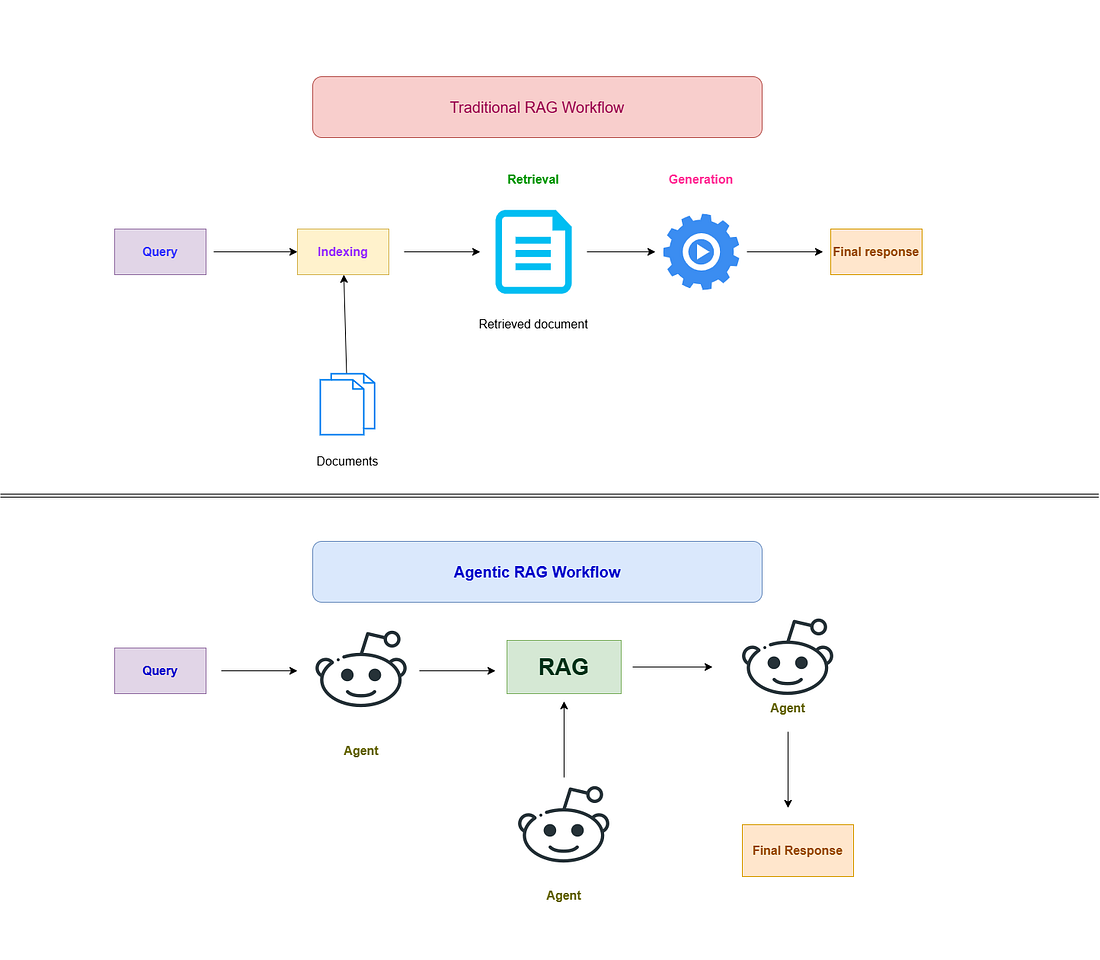
\includegraphics[width=0.92\textwidth]{figures/AgenticRAG.png}
  \source{Figure reprise du dossier du projet, inspirée de l'article Medium sur l'Agentic RAG \cite{nimeesha2024agenticrag}}
\end{figure}

La figure \ref{fig:rag_graphrag_agentic_rag} illustre la rupture entre une \RAG{} traditionnelle et une architecture agentique. Dans le flux traditionnel, la requête traverse une chaîne relativement fixe : indexation, récupération d'un document, génération, puis réponse finale. Dans le flux agentique, la requête passe par un ou plusieurs agents capables de coordonner la récupération, de solliciter plusieurs outils et d'organiser la réponse. L'image met surtout en évidence que l'Agentic RAG n'est pas seulement une meilleure recherche documentaire ; c'est une organisation dynamique de la recherche et de la génération.

\section{Agentic RAG}

L'Agentic RAG désigne une extension de la \RAG{} dans laquelle la récupération n'est plus une étape fixe et unique, mais une séquence pilotée par un agent. L'idée, mise en avant dans les travaux récents sur les agents outillés et illustrée dans des synthèses techniques comme l'article Medium consulté \cite{nimeesha2024agenticrag}, est de remplacer une chaîne linéaire \og requête--recherche--génération \fg{} par une boucle plus adaptative : planifier, appeler un outil, observer le résultat, décider si l'information est suffisante, puis continuer ou produire la réponse. Cette logique rejoint les modèles de raisonnement-action tels que ReAct, où un modèle alterne raisonnement et usage d'outils externes \cite{yao2023react}.

La différence avec une \RAG{} classique est importante. Dans une \RAG{} standard, la stratégie de récupération est déterminée à l'avance : le système récupère, par exemple, les dix documents les plus proches puis génère une réponse. Dans un Agentic RAG, le système peut décider que les documents récupérés sont insuffisants, reformuler la requête, interroger une autre base, vérifier une contrainte ou demander un calcul complémentaire. Des approches comme Self-RAG montrent également l'intérêt d'introduire des mécanismes de critique ou d'auto-vérification afin de décider quand récupérer de l'information et comment contrôler la génération \cite{asai2024selfrag}.

Son fonctionnement repose donc sur quatre composantes. La première est un planificateur, qui transforme l'objectif utilisateur en étapes : chercher, vérifier, comparer, expliquer. La deuxième est une bibliothèque d'outils, par exemple une base vectorielle, un graphe de connaissances, un module de scoring ou une API métier. La troisième est une mémoire ou une trace d'exécution, qui conserve les observations produites à chaque étape. La quatrième est un module de contrôle, qui vérifie si la réponse est suffisamment fondée avant de la présenter. Sans ce contrôle, l'agentivité devient un risque : le système peut multiplier les actions sans améliorer la vérité de la réponse.

Dans le cadre du matching emploi-compétences, l'Agentic RAG ne doit pas être compris comme un agent libre qui \og pense \fg{} à la place de l'expert. Ce serait méthodologiquement fragile. Il doit plutôt être conçu comme une orchestration contrôlée de fonctions spécialisées. Le système peut, par exemple, recevoir l'objectif suivant : recommander des offres accessibles à un candidat et proposer une trajectoire de montée en compétences. L'agent transforme alors cet objectif en un plan opérationnel :

\begin{enumerate}
    \item récupérer le profil normalisé du candidat;
    \item rechercher les offres proches dans la base vectorielle \texttt{pgvector};
    \item vérifier dans Neo4j les contraintes de niveau \NCF{}, de secteur, de localisation et de compétences;
    \item calculer le \emph{skill gap} pour les offres présélectionnées;
    \item pénaliser les offres présentant trop de compétences essentielles manquantes;
    \item générer une justification fondée sur les scores, les relations du graphe et les formations associées.
\end{enumerate}

La plus-value est donc différente de celle d'un simple modèle de langue. Un Agentic RAG apporte une capacité d'orchestration : il combine recherche sémantique, interrogation du graphe, calcul de score, contrôle des contraintes et verbalisation finale. Dans un système emploi-formation, cette orchestration est précieuse parce que la bonne recommandation n'est pas nécessairement l'offre textuellement la plus proche. Elle est l'offre dont la proximité sémantique, la compatibilité institutionnelle, les compétences requises et les possibilités de formation forment un ensemble cohérent.

Pour éviter l'effet de mode, il faut toutefois poser des limites claires. Un Agentic RAG n'améliore pas automatiquement la qualité d'un système. S'il appelle de mauvais outils, s'il dispose d'un graphe incomplet ou s'il n'enregistre pas ses décisions, il peut produire des recommandations plus complexes mais pas plus fiables. Dans ce mémoire, l'agentivité doit donc être envisagée comme une couche cible d'orchestration explicable : les scores restent calculés par le code, les contraintes sont vérifiées dans les données, les chemins de graphe sont traçables, et le \LLM{} sert à organiser et formuler la réponse. Cette position est plus défendable qu'une présentation vague où l'agent serait supposé prendre de meilleures décisions par lui-même.

Appliquée au projet, la logique Agentic RAG peut être résumée ainsi : le modèle d'embeddings propose des candidats, le graphe vérifie et explique, le module de scoring classe, le générateur rédige, et l'agent coordonne la séquence en fonction de l'objectif. La valeur ajoutée scientifique tient alors à l'articulation entre représentation vectorielle, raisonnement relationnel et contrôle génératif ; la valeur ajoutée opérationnelle tient à la capacité d'expliquer non seulement quelle offre est recommandée, mais aussi pourquoi elle est accessible, quelles compétences manquent et quelles formations peuvent réduire cet écart.


\chapter{Approche méthodologique et données}
\vspace{-1.4cm}

\section{Positionnement méthodologique}

L'approche méthodologique retenue est une démarche de conception d'artefact appliquée au problème d'appariement entre offres d'emploi, profils de demandeurs, compétences, métiers et formations. Elle ne se limite donc pas à l'entraînement d'un modèle statistique isolé. Elle combine trois niveaux complémentaires : la préparation des données, l'apprentissage de représentations sémantiques et la structuration relationnelle des connaissances dans un graphe.

L'étude adopte une architecture cible de type GraphRAG, dans laquelle un encodeur sémantique permet de retrouver les offres ou profils proches, tandis qu'un graphe de connaissances apporte le contexte métier, les relations entre compétences et les trajectoires de formation. Dans le cadre du présent travail, la démarche mise en œuvre couvre trois composantes principales : la préparation des données, l'adaptation d'un modèle d'embeddings au domaine emploi-compétences et la construction d'un graphe de connaissances intégrant les référentiels \ESCO{}, \MEPC{} et \NCF{}. Les composantes relatives à l'orchestration générative complète, à l'exposition applicative et à l'évaluation utilisateur relèvent de la continuité du système et ne sont pas présentées comme des résultats entièrement achevés.

Cette distinction est importante. Elle évite de confondre l'architecture conceptuelle du système avec son état d'implémentation. La méthodologie ci-dessous décrit donc factuellement ce qui a été réalisé, puis précise les extensions prévues pour aboutir à un système de recommandation hybride complet \cite{reimers2019sbert,hogan2021knowledge,lewis2020rag,burke2002hybrid,ricci2011recommender}.

\begin{figure}[H]
  \centering
  \caption{Vue d'ensemble de l'approche méthodologique du système hybride emploi-compétences}
  \label{fig:approche_methodologique}
  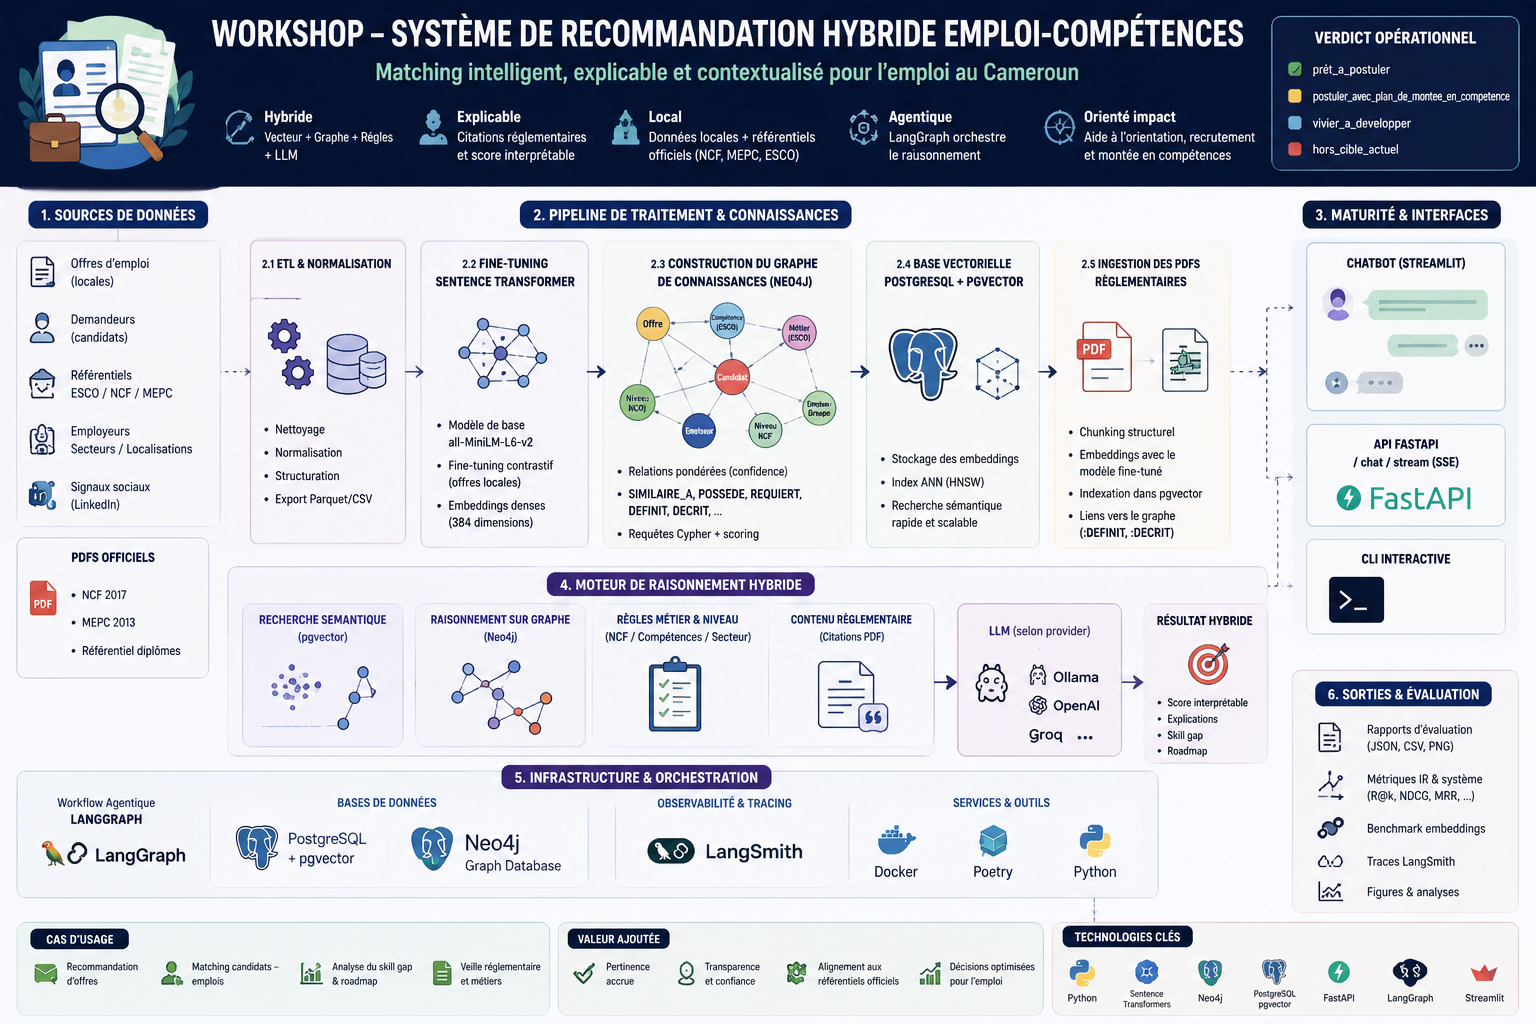
\includegraphics[width=0.98\textwidth]{figures/approche.png}
  \source{Auteur}
\end{figure}

La figure~\ref{fig:approche_methodologique} synthétise le positionnement méthodologique du mémoire. Elle montre que la solution n'est pas un simple moteur de recherche par mots-clés, ni un modèle de langage utilisé directement comme oracle. Le système est conçu comme une chaîne hybride où chaque brique a une fonction contrôlable : les données locales alimentent l'ETL, les textes normalisés alimentent l'encodeur sémantique, le graphe conserve les relations métiers et institutionnelles, la base vectorielle permet la recherche rapide de similarité, les documents réglementaires apportent des preuves textuelles, puis le moteur de raisonnement combine ces signaux avant l'exposition dans des interfaces opérationnelles.

\subsection*{Déclinaison des briques de la solution}

\paragraph{Sources de données.}
La première brique correspond aux données brutes mobilisées pour représenter le marché du travail. Elle comprend les offres d'emploi locales, les profils de demandeurs, les référentiels \ESCO{}, \NCF{} et \MEPC{}, les informations sur les employeurs, les secteurs et les localisations, ainsi que certains signaux sociaux. Son rôle méthodologique est de couvrir simultanément la demande de travail, l'offre de travail et les nomenclatures nécessaires à leur comparaison. Le point critique est la qualité de ces sources : si les compétences sont mal renseignées ou si les intitulés de métiers sont trop ambigus, aucun modèle avancé ne pourra corriger entièrement cette faiblesse en aval.

\paragraph{ETL et normalisation.}
La deuxième brique transforme les sources hétérogènes en tables exploitables. Elle nettoie les champs textuels, harmonise les formats, déduplique les annonces, extrait les listes de compétences, rapproche les niveaux de formation de la \NCF{} et produit des fichiers structurés en Parquet, CSV ou JSONL. Cette étape est méthodologiquement décisive, car elle fixe l'unité d'observation du système : offre, candidat, compétence, métier, formation, secteur, employeur ou localisation. Une recommandation fiable suppose donc que ces unités soient stables, identifiables et comparables.

\paragraph{Fine-tuning du modèle Sentence Transformer.}
La troisième brique adapte un encodeur sémantique au domaine emploi-compétences. Le projet part d'un modèle Sentence Transformer pré-entraîné, puis l'ajuste par apprentissage contrastif sur des paires construites à partir des offres locales. L'objectif n'est pas de pré-entraîner un \LLM{} depuis zéro, mais d'obtenir des embeddings plus sensibles au vocabulaire des annonces, des métiers, des compétences et des niveaux de qualification. Les vecteurs produits servent ensuite à mesurer la proximité sémantique entre candidats, offres, compétences et référentiels \cite{reimers2019sbert}.

\paragraph{Construction du graphe de connaissances.}
La quatrième brique organise les entités et leurs relations dans Neo4j. Les nœuds représentent notamment les candidats, les offres, les compétences \ESCO{}, les métiers \ESCO{}, les niveaux \NCF{}, les groupes \MEPC{}, les secteurs, les employeurs et les localisations. Les relations expriment des liens interprétables : un candidat \textit{possède} une compétence, une offre \textit{requiert} une compétence, un métier est \textit{aligné} sur un référentiel, un document \textit{décrit} ou \textit{définit} un élément réglementaire. Cette brique donne au système une capacité d'explication que la seule similarité vectorielle ne fournit pas : elle permet de justifier le résultat par des chemins, des relations et des contraintes métiers \cite{hogan2021knowledge}.

\paragraph{Base vectorielle PostgreSQL et pgvector.}
La cinquième brique stocke les embeddings dans PostgreSQL à travers l'extension pgvector. Elle permet de retrouver rapidement les entités les plus proches dans l'espace sémantique, par exemple les offres les plus proches d'un profil ou les compétences proches d'un besoin exprimé librement. Le rôle de cette brique est la scalabilité de la recherche. Le graphe est fort pour raisonner sur les relations ; la base vectorielle est forte pour retrouver rapidement des contenus proches dans un grand volume de textes.

\paragraph{Ingestion des PDF réglementaires.}
La sixième brique traite les documents officiels, notamment la \NCF{}, la \MEPC{} et les référentiels de diplômes. Ces PDF sont découpés en segments structurés, transformés en embeddings, indexés dans pgvector et reliés au graphe. Cette étape évite que le système se contente d'une réponse plausible : lorsqu'une recommandation mobilise un niveau de formation, un domaine ou un métier réglementé, elle peut être reliée à un passage documentaire exploitable. C'est une condition importante pour une recommandation explicable et vérifiable.

\paragraph{Moteur de raisonnement hybride.}
La septième brique combine les signaux au lieu d'en privilégier un seul. La recherche sémantique propose des candidats proches ; le graphe vérifie les relations et les contraintes ; les règles métier contrôlent les niveaux de formation, les compétences et les secteurs ; les contenus réglementaires apportent des citations ; le \LLM{} intervient pour formuler une réponse structurée lorsque le mode génératif est activé. Le résultat attendu est un score interprétable, une explication, un \emph{skill gap} et une feuille de route de montée en compétence. C'est précisément ici que se situe le caractère hybride du système \cite{burke2002hybrid,ricci2011recommender}.

\paragraph{Infrastructure, orchestration et interfaces.}
La huitième brique correspond à l'environnement d'exécution : Python et Poetry pour la reproductibilité, PostgreSQL/pgvector et Neo4j pour les bases de données, LangSmith pour le traçage, FastAPI pour l'exposition des endpoints, Streamlit pour le chatbot et LangGraph pour l'orchestration agentique. Cette couche ne doit pas être confondue avec le cœur scientifique du modèle, mais elle conditionne son usage réel. Un système de recommandation qui ne peut pas être interrogé, tracé et testé reste un prototype fragile.

\paragraph{Sorties et évaluation.}
La dernière brique transforme le raisonnement en résultats contrôlables : recommandations d'offres, matching candidats--emplois, analyse du \emph{skill gap}, roadmap de formation, rapports d'évaluation, métriques de recherche d'information et traces d'exécution. Cette brique ferme la boucle méthodologique. Elle permet de juger le système sur des sorties observables plutôt que sur une intention de conception. Elle impose aussi une discipline : une recommandation n'est acceptable que si son score, ses preuves, ses limites et ses écarts de compétences peuvent être inspectés.

Ainsi, l'approche méthodologique retenue est défendable parce qu'elle sépare clairement les responsabilités. Le modèle d'embeddings sert à la proximité sémantique ; Neo4j sert à la structure relationnelle ; pgvector sert à l'indexation vectorielle ; les référentiels servent à l'ancrage institutionnel ; les règles métier servent au contrôle ; le \LLM{} sert à la génération explicative ; l'orchestration agentique sert à coordonner ces opérations. Cette séparation réduit le risque de construire une boîte noire où une réponse générée serait acceptée sans preuve. Elle rend au contraire possible un système de recommandation plus auditable, plus localisé et plus utile pour l'orientation, le recrutement et la montée en compétences.

\section{Sources de données mobilisées}

Le projet s'appuie sur deux familles de données. La première correspond aux données opérationnelles du marché du travail : offres d'emploi et profils de demandeurs. Les offres d'emploi ont été collectées par KmerAI à partir d'un dispositif de scraping mis en place sur des sites partenaires de diffusion d'annonces. Cette collecte a permis de constituer une base décrivant la demande de travail à travers les intitulés de poste, les secteurs d'activité, les localisations, les employeurs, les niveaux d'étude attendus, les compétences mentionnées et les descriptions textuelles des annonces. Les données de demandeurs décrivent, quant à elles, l'offre de travail disponible : profil, niveau de formation, diplôme, spécialité, expérience, mobilité et objectif professionnel.

La seconde famille de données correspond aux référentiels de structuration. Le référentiel \ESCO{} apporte une nomenclature internationale de métiers, de compétences et de relations métier--compétence. La \MEPC{} et la \NCF{}, produites par l'Institut National de la Statistique du Cameroun, permettent d'ancrer l'analyse dans le contexte institutionnel camerounais. Dans le projet, ces deux nomenclatures nationales étaient initialement disponibles sous forme de documents PDF. Elles ont donc été organisées avant leur exploitation : extraction des rubriques, nettoyage des libellés, reconstitution des codes, séparation des niveaux hiérarchiques et transformation en tables structurées. Cette étape est méthodologiquement centrale, car une nomenclature en PDF est lisible pour un humain, mais elle n'est pas directement interrogeable par un système de recommandation.

\begin{table}[H]
  \centering
  \caption{Sources de données utilisées dans le projet}
  \label{tab:sources_methodologie}
  \footnotesize
  \begin{tabularx}{\textwidth}{p{3.2cm}X p{3.2cm}}
    \toprule
    \textbf{Source} & \textbf{Rôle méthodologique} & \textbf{Utilisation dans le projet} \\
    \midrule
    Offres d'emploi scrapées par KmerAI & Décrire la demande de travail : intitulé, secteur, localisation, employeur, niveau d'étude, compétences et contenu textuel de l'annonce. & Normalisation, génération du texte d'embedding, construction des paires de fine-tuning et création des nœuds d'offres. \\
    Demandeurs d'emploi & Décrire l'offre de travail : profil, diplôme, niveau d'étude, expérience, compétences et mobilité. & Normalisation des profils et rattachement aux niveaux de formation. \\
    \ESCO{} & Fournir une nomenclature internationale de métiers, compétences et relations métier--compétence. & Chargement des occupations, compétences, groupes ISCO et relations occupation--compétence. \\
    \MEPC{} -- INS Cameroun & Fournir une classification nationale des métiers, emplois et professions du Cameroun. & Organisation du PDF en grands groupes, sous-groupes et groupes de base, puis alignement avec les métiers \ESCO{}. \\
    \NCF{} -- INS Cameroun & Fournir une nomenclature nationale des niveaux, domaines et spécialités de formation. & Organisation du PDF en niveaux, grands domaines, domaines spécialisés et domaines détaillés, puis rattachement aux profils et aux offres. \\
    \bottomrule
  \end{tabularx}
  \source{Auteur}
\end{table}

La méthodologie tient compte de l'hétérogénéité terminologique du marché du travail camerounais, notamment les variations d'intitulés de postes, les écarts entre libellés de compétences et les différences de granularité entre référentiels. Cette difficulté est traitée par une standardisation progressive : nettoyage des textes, construction de champs normalisés, alignement partiel des référentiels et représentation du résultat dans un graphe de connaissances.

\section{Pipeline de préparation des données}

La préparation des données est organisée autour de quatre étapes principales : la normalisation des offres, la normalisation des candidats, l'organisation des référentiels et la construction des paires d'entraînement. Cette organisation permet de transformer des données initialement hétérogènes en informations exploitables par le modèle sémantique, la base vectorielle et le graphe de connaissances.

Concrètement, la chaîne de traitement part de fichiers bruts de nature différente : annonces d'emploi collectées par scraping, fichier de demandeurs, fichiers \ESCO{} en format tabulaire et documents PDF issus de l'INS Cameroun pour la \MEPC{} et la \NCF{}. Ces sources ne sont pas directement comparables. Les annonces utilisent des libellés libres ; les profils candidats contiennent des diplômes et objectifs parfois incomplets ; les référentiels nationaux ont une structure hiérarchique mais initialement non exploitable automatiquement. Le travail de préparation consiste donc à produire une couche intermédiaire standardisée : identifiants stables, libellés nettoyés, listes de compétences, niveaux \NCF{}, tables hiérarchiques de nomenclature, textes d'embedding et tables de correspondance.

\subsection{Normalisation des offres}

La normalisation des offres vise à transformer des annonces scrapées, souvent hétérogènes dans leur forme, en variables exploitables par le modèle et par le graphe. Le traitement commence par l'identification des annonces redondantes à partir d'une clé composée du titre du poste, de l'employeur, de la ville et du secteur. L'objectif est de limiter les doublons produits par la reprise d'une même annonce sur plusieurs pages ou par des variations mineures dans le contenu collecté.

Après cette déduplication, les champs textuels sont harmonisés. Les espaces inutiles, les caractères parasites, les formulations de scraping et les blocs répétitifs sont réduits. Les champs multi-valeurs sont ensuite séparés : les villes deviennent une liste de localisations avec une ville principale, les secteurs deviennent une liste de secteurs avec un secteur principal, et les compétences sont transformées en liste de compétences déclarées. Cette étape est importante, car une valeur comme \og Douala/Yaoundé \fg{} ou \og Informatique; Télécom; Réseaux \fg{} ne doit pas rester une seule chaîne confuse dans la base.

Un champ textuel synthétique est ensuite construit pour représenter chaque offre sous forme de contenu exploitable par un encodeur sémantique. Ce champ ne doit pas être compris comme une simple concaténation mécanique. Il joue le rôle d'une fiche normalisée de l'offre, dans laquelle les compétences requises, le détail nettoyé de l'annonce et les éléments de contexte sont rapprochés afin que le modèle puisse apprendre les correspondances entre intitulés, secteurs, compétences et exigences de qualification.

En parallèle, une chaîne courte de métadonnées est créée pour chaque offre. Elle rassemble les informations utiles côté requête : poste, secteur, type de contrat, niveau d'étude, expérience et ville. Le projet dispose ainsi de deux représentations complémentaires : un texte riche décrivant le contenu de l'offre et une représentation structurée plus courte décrivant ses métadonnées principales.

Une attention particulière est portée au niveau de formation. Les niveaux indiqués dans les offres sont rapprochés de la \NCF{} afin de produire des codes de formation plus homogènes. Le résultat final des offres normalisées contient notamment les champs \textit{offre\_id}, \textit{source}, \textit{titre\_poste}, \textit{employeur}, \textit{pays}, \textit{ville\_principale}, \textit{villes\_list}, \textit{secteur\_principal}, \textit{secteurs\_list}, \textit{type\_contrat\_norm}, \textit{ncf\_niveau\_code}, \textit{experience\_min\_ans}, \textit{skills\_list}, \textit{skills\_raw}, \textit{details\_clean}, \textit{text\_to\_embed}, \textit{metadata\_str} et \textit{ft\_eligible}. Cette étape est essentielle, car la recommandation ne doit pas seulement rapprocher des textes : elle doit aussi vérifier que le profil du candidat est compatible avec les exigences de qualification.

\subsection{Normalisation des candidats}

La normalisation des candidats suit la même logique. Les informations disponibles sur le niveau d'étude, le diplôme, l'expérience, les compétences, le secteur demandé, la qualification visée et la mobilité sont harmonisées. Le projet produit un niveau \NCF{} final pour les candidats lorsque l'information disponible le permet. Cette variable sert ensuite à comparer les profils aux exigences des offres et à préparer les relations dans le graphe.

Deux sources d'information sont mobilisées pour stabiliser ce niveau : le niveau d'étude déclaré et le diplôme. Lorsque le diplôme apporte une information plus précise, il est prioritaire sur le niveau général. La mobilité géographique est transformée en indicateur booléen et, lorsque c'est possible, en liste de villes. Les valeurs non déclarées sont traitées comme des informations manquantes plutôt que comme de vraies modalités statistiques.

Le résultat final des candidats normalisés contient notamment les champs \textit{candidat\_id}, \textit{age}, \textit{genre}, \textit{diplome\_raw}, \textit{ncf\_niveau\_final}, \textit{ncf\_code\_niveau\_etude}, \textit{ncf\_code\_diplome}, \textit{niveau\_etude\_raw}, \textit{qualification\_metier}, \textit{secteur\_metier}, \textit{filiere\_specialite}, \textit{secteur\_demande}, \textit{metier\_vise}, \textit{objectif}, \textit{mobilite\_geo\_bool}, \textit{mobilite\_geo\_villes} et \textit{text\_to\_embed}. Le traitement ne prétend pas résoudre toute l'ambiguïté des parcours individuels. Un diplôme ou un niveau d'étude peut être formulé de manière imprécise, et certains profils peuvent cumuler plusieurs formations. La méthode adoptée est donc pragmatique : elle crée une variable normalisée utilisable par le système, tout en conservant la nécessité d'une validation métier pour les cas ambigus.

\subsection{Alignement des référentiels}

L'alignement des référentiels concerne trois sources : \ESCO{}, \MEPC{} et \NCF{}. \ESCO{} apporte une base internationale structurée autour des métiers, compétences et groupes ISCO. La \MEPC{} permet d'ancrer les métiers dans la nomenclature nationale camerounaise. La \NCF{} apporte une structure pour les niveaux et domaines de formation. Le passage des documents PDF \MEPC{} et \NCF{} de l'INS Cameroun à des tables structurées a consisté à identifier la hiérarchie interne de chaque nomenclature, à isoler les codes et les intitulés, puis à créer des niveaux séparés afin que chaque élément puisse devenir un nœud ou une propriété dans la base graphe.

Pour la \MEPC{}, la structuration retient notamment trois niveaux : \textit{GrandGroupeMEPC}, \textit{SousGroupeMEPC} et \textit{GroupeBaseMEPC}. Pour la \NCF{}, la structuration retient quatre niveaux : \textit{NiveauFormationNCF}, \textit{GrandDomaineNCF}, \textit{DomaineSpécialiséNCF} et \textit{DomaineDétailléNCF}. Cette séparation évite de réduire les référentiels nationaux à de simples libellés. Elle permet de préserver leur hiérarchie et de les exploiter dans les raisonnements de recommandation.

Dans l'état actuel du projet, l'alignement entre \MEPC{} et \ESCO{} repose sur une correspondance pragmatique à partir des préfixes de codes ISCO/CITP lorsque ces codes sont disponibles. Cette stratégie augmente la couverture, mais elle ne constitue pas une preuve d'équivalence métier parfaite. Deux métiers peuvent partager un même préfixe de classification tout en différant par leurs compétences fines, leur niveau de responsabilité ou leur contexte sectoriel. Cette limite doit être explicitement conservée dans l'interprétation des résultats.

\subsection{Structure finale des tables \MEPC{} et \NCF{} issues des PDF}

La transformation des PDF \MEPC{} et \NCF{} n'a pas consisté à produire une simple copie numérique du document. Le travail a consisté à obtenir des tables directement exploitables par le graphe Neo4j et par la base vectorielle. Chaque ligne devait donc posséder un identifiant, un libellé, une information hiérarchique et un texte descriptif utilisable pour l'embedding.

\begin{table}[H]
  \centering
  \caption{Structure finale des tables \MEPC{} issues du PDF de l'INS Cameroun}
  \label{tab:structure_mepc_finale}
  \footnotesize
  \begin{tabularx}{\textwidth}{p{3.4cm}p{4.1cm}X}
    \toprule
    \textbf{Table finale} & \textbf{Unité statistique} & \textbf{Champs structurants} \\
    \midrule
    \textit{mepc\_grands\_groupes} & Grand groupe de métiers & \textit{code}, \textit{intitule}, \textit{notes\_explicatives}, \textit{codes\_citp}, \textit{text\_to\_embed}. \\
    \textit{mepc\_sous\_groupes} & Sous-groupe rattaché à un grand groupe & \textit{code}, \textit{intitule}, \textit{notes\_explicatives}, \textit{codes\_citp}, \textit{code\_grand\_groupe}, \textit{text\_to\_embed}. \\
    \textit{mepc\_groupes\_base} & Groupe de base, niveau le plus fin retenu pour le matching métier & \textit{code}, \textit{intitule}, \textit{notes\_explicatives}, \textit{codes\_citp}, \textit{code\_sous\_groupe}, \textit{code\_grand\_groupe}, \textit{text\_to\_embed}. \\
    \bottomrule
  \end{tabularx}
  \source{Auteur, à partir de la \MEPC{} de l'INS Cameroun}
\end{table}

Dans cette structure, le champ \textit{code} sert d'identifiant de référence. Le champ \textit{intitule} conserve le libellé métier officiel. Les \textit{notes\_explicatives} apportent le contexte descriptif de la catégorie. Les \textit{codes\_citp} servent de passerelle avec les groupes ISCO et donc avec \ESCO{}. Les champs \textit{code\_grand\_groupe} et \textit{code\_sous\_groupe} permettent de reconstruire la hiérarchie \MEPC{} dans Neo4j par des relations \textit{CONTIENT}. Enfin, \textit{text\_to\_embed} regroupe le libellé et les notes utiles pour représenter chaque catégorie métier sous forme vectorielle.

\begin{table}[H]
  \centering
  \caption{Structure finale des tables \NCF{} issues du PDF de l'INS Cameroun}
  \label{tab:structure_ncf_finale}
  \footnotesize
  \begin{tabularx}{\textwidth}{p{3.5cm}p{4cm}X}
    \toprule
    \textbf{Table finale} & \textbf{Unité statistique} & \textbf{Champs structurants} \\
    \midrule
    \textit{ncf\_niveaux} & Niveau de formation & \textit{code}, \textit{intitule}, \textit{explication}, \textit{text\_to\_embed}. \\
    \textit{ncf\_grands\_domaines} & Grand domaine de formation & \textit{code}, \textit{intitule}, \textit{explication}, \textit{text\_to\_embed}. \\
    \textit{ncf\_dom\_specialises} & Domaine spécialisé rattaché à un grand domaine & \textit{code}, \textit{intitule}, \textit{explication}, \textit{code\_grand\_domaine}, \textit{text\_to\_embed}. \\
    \textit{ncf\_dom\_detailles} & Domaine détaillé, niveau le plus fin retenu pour rattacher les formations & \textit{code}, \textit{intitule}, \textit{explication}, \textit{code\_dom\_specialise}, \textit{code\_grand\_domaine}, \textit{text\_to\_embed}. \\
    \bottomrule
  \end{tabularx}
  \source{Auteur, à partir de la \NCF{} de l'INS Cameroun}
\end{table}

La \NCF{} est donc exploitée à deux niveaux. Le premier niveau concerne la qualification minimale ou déclarée : il permet de relier une offre ou un candidat à un \textit{NiveauFormationNCF}. Le second niveau concerne le domaine de formation : il permet de relier un profil à un \textit{DomaineDétailléNCF} lorsque la filière ou la spécialité est suffisamment explicite. Cette distinction est importante, car deux candidats peuvent avoir le même niveau de formation tout en appartenant à des domaines très différents.

Une table de correspondance complémentaire relie ensuite la \MEPC{} à \ESCO{}. Elle contient notamment \textit{mepc\_code\_base}, \textit{mepc\_intitule}, \textit{code\_sous\_groupe}, \textit{code\_grand\_groupe}, \textit{codes\_citp}, \textit{isco\_code\_mepc}, \textit{esco\_uri}, \textit{esco\_label} et \textit{esco\_isco\_code}. Son rôle est de rapprocher les groupes de base de la \MEPC{} des métiers \ESCO{} en passant par les codes CITP/ISCO disponibles. Ce rapprochement doit être lu comme un alignement de travail, utile pour augmenter la couverture du graphe, mais non comme une équivalence parfaite entre nomenclatures.

\subsection{Construction des paires de fine-tuning}

Les paires de fine-tuning sont construites à partir des offres jugées exploitables, c'est-à-dire celles dont les champs textuels sont suffisamment renseignés pour permettre un apprentissage contrastif. Ce filtre ne constitue pas une mesure de qualité économique de l'offre ; il indique seulement que l'observation contient assez d'information pour être utilisée dans l'adaptation du modèle sémantique.

Chaque paire associe une requête structurée, composée de métadonnées, à un texte cible composé des compétences et des détails nettoyés de l'offre. Le côté requête correspond à \textit{metadata\_str} : poste, secteur, contrat, niveau d'étude, expérience et ville. Le côté corpus correspond à \textit{text\_to\_embed} : compétences requises et description nettoyée de l'annonce. Le système ne conserve que les paires dont les deux côtés ont une longueur minimale suffisante, afin d'éviter d'entraîner le modèle sur des observations trop pauvres.

Le corpus obtenu comprend 3\,302 paires au total, réparties en 2\,321 paires d'entraînement, 508 paires de validation et 473 paires de test, selon une partition 70/15/15 avec une graine aléatoire fixée à 42. La séparation est effectuée en tenant compte du secteur principal afin de limiter le risque d'avoir un jeu d'entraînement dominé par quelques secteurs seulement. Cette précaution est importante dans un marché où les annonces peuvent être plus nombreuses dans la distribution, les TIC, la banque ou le marketing que dans d'autres domaines.

\section{Fine-tuning du SentenceTransformer}

La deuxième phase du projet correspond à l'adaptation d'un modèle d'embeddings au vocabulaire des offres d'emploi. L'objectif n'est pas de fine-tuner un modèle génératif pour produire du texte, mais d'améliorer un modèle de représentation sémantique afin qu'il place, dans un même espace vectoriel, les requêtes d'emploi et les descriptions d'offres qui se correspondent réellement. Cette distinction est importante : le modèle n'apprend pas à rédiger une annonce ; il apprend à mieux rapprocher une intention de recherche, un profil ou une fiche synthétique d'offre avec le contenu détaillé d'une annonce.

La composante sémantique repose sur le modèle \texttt{all-MiniLM-L6-v2}, un SentenceTransformer produisant des embeddings de dimension 384. Ce modèle a été retenu parce qu'il offre un compromis raisonnable entre qualité de représentation, coût de calcul et vitesse d'indexation. Dans le cadre du mémoire, il sert de bi-encodeur : une première phrase est encodée côté requête, une seconde phrase est encodée côté document, puis la proximité est mesurée par similarité cosinus. Cette logique est cohérente avec les modèles de type Sentence-BERT, conçus pour comparer efficacement des phrases ou documents dans un espace vectoriel commun \cite{reimers2019sbert}.

\subsection{Problème d'apprentissage retenu}

Le fine-tuning est formulé comme un problème de recherche d'information. Pour chaque offre d'emploi, le système construit une paire positive composée de deux vues complémentaires de la même annonce. La première vue, appelée \textit{sentence1}, correspond aux métadonnées structurées : titre du poste, secteur, type de contrat, niveau d'étude, expérience et ville. La seconde vue, appelée \textit{sentence2}, correspond au contenu textuel plus riche : compétences requises et détails nettoyés de l'annonce.

Ce choix méthodologique répond à une contrainte réelle du système. Au moment de la recommandation, une requête candidat ou une fiche de besoin n'a pas toujours la même forme qu'une annonce complète. Elle ressemble davantage à une description courte et structurée. Le modèle doit donc apprendre qu'une requête telle que \og poste data analyst, secteur TIC, niveau licence, ville Douala \fg{} peut être proche d'une annonce longue mentionnant Python, SQL, reporting, tableaux de bord et analyse statistique, même si les formulations ne sont pas identiques.

Ainsi, chaque paire positive peut être interprétée comme suit :

\begin{equation}
(\text{métadonnées structurées de l'offre},\ \text{description riche de l'offre})
\end{equation}

La stratégie n'utilise donc pas des labels manuels de pertinence profil--offre. Elle exploite une supervision faible mais cohérente : les deux textes proviennent de la même annonce et doivent être proches dans l'espace vectoriel. Cette approche est adaptée lorsque les données annotées par experts sont rares, mais que l'on dispose d'un volume suffisant d'annonces normalisées.

\subsection{Préparation du corpus de fine-tuning}

Les paires ne sont pas construites sur toutes les offres brutes. Une offre est retenue uniquement si elle contient assez d'information des deux côtés : des métadonnées suffisamment renseignées et une description exploitable. Le filtre \textit{ft\_eligible} vérifie donc la longueur minimale de \textit{metadata\_str} et de \textit{text\_to\_embed}. Ce filtre n'est pas un jugement sur la qualité économique de l'offre ; il indique seulement que l'observation est utilisable pour l'apprentissage contrastif.

Le corpus final comprend 3\,302 paires. Les métadonnées structurées ont une longueur moyenne d'environ 159 caractères, tandis que les textes riches ont une longueur moyenne d'environ 559 caractères. Cette asymétrie est volontaire : le modèle apprend à rapprocher une requête courte d'un document plus détaillé. Les paires sont réparties en 2\,321 observations d'entraînement, 508 de validation et 473 de test, selon une partition 70/15/15 avec une graine aléatoire fixée à 42. La partition tient compte du secteur principal afin de limiter une concentration excessive des mêmes familles d'offres dans un seul sous-ensemble.

\subsection{Fonction de perte et logique contrastive}

L'entraînement repose sur une fonction de perte contrastive de type \texttt{MultipleNegativesRankingLoss}. Cette perte est adaptée aux tâches de recherche sémantique : pour une paire positive, les autres éléments du batch jouent le rôle de négatifs implicites. Le modèle apprend ainsi à donner un score élevé à la paire correcte et un score plus faible aux associations non pertinentes.

Plus précisément, dans un batch de taille 32, chaque paire $(q_i,d_i)$ est considérée comme positive, où $q_i$ représente la requête structurée et $d_i$ le texte détaillé correspondant. Les documents $d_j$ des autres paires du même batch, avec $j \neq i$, sont utilisés comme négatifs implicites. Le modèle doit donc maximiser la similarité cosinus entre $q_i$ et $d_i$, tout en réduisant la similarité entre $q_i$ et les autres documents du batch. Cette stratégie est efficace parce qu'elle évite de construire manuellement des exemples négatifs, opération coûteuse et souvent ambiguë dans le domaine emploi-compétences.

La logique d'optimisation peut être résumée par l'idée suivante : pour une requête donnée, le bon document doit être mieux classé que les documents concurrents présents dans le batch. Le fine-tuning agit donc directement sur le comportement de ranking du modèle, et non sur une simple classification binaire.

\subsection{Paramètres d'entraînement}

\begin{table}[H]
  \centering
  \caption{Paramètres du fine-tuning sémantique}
  \label{tab:parametres_finetuning}
  \footnotesize
  \begin{tabularx}{\textwidth}{p{4.2cm}X}
    \toprule
    \textbf{Paramètre} & \textbf{Valeur utilisée} \\
    \midrule
    Modèle de base & \texttt{all-MiniLM-L6-v2} \\
    Dimension des embeddings & 384 \\
    Fonction de perte & \texttt{MultipleNegativesRankingLoss} \\
    Nombre d'époques & 5 \\
    Taille de batch & 32 \\
    Taux d'apprentissage & $2 \times 10^{-5}$ \\
    Temps d'entraînement & 6\,630,9 secondes \\
    Données d'entraînement & 2\,321 paires \\
    Données de validation & 508 paires \\
    Données de test & 473 paires \\
    Critère de sélection & \texttt{val-information-retrieval\_cosine\_ndcg@10} \\
    \bottomrule
  \end{tabularx}
  \source{Auteur}
\end{table}

Le taux d'apprentissage de $2 \times 10^{-5}$ est volontairement modéré. Dans un fine-tuning de modèle pré-entraîné, l'objectif n'est pas de réapprendre toute la langue, mais d'ajuster l'espace vectoriel au domaine des offres d'emploi. Un taux trop élevé aurait pu dégrader les représentations générales déjà acquises par le modèle. Les cinq époques permettent d'observer la progression du modèle tout en gardant un risque de sur-apprentissage contrôlé par le suivi des métriques de validation.

\subsection{Validation et choix du modèle}

L'évaluation du modèle est réalisée comme une tâche de retrieval. Pour chaque requête de validation ou de test, le système classe les textes candidats selon la similarité cosinus et vérifie si le texte associé à la bonne offre apparaît dans les premiers résultats. Les métriques utilisées sont Recall@K, NDCG@K, MRR@K et MAP@K. Elles sont plus adaptées qu'une simple précision globale, car l'enjeu opérationnel est de produire une liste courte d'offres pertinentes.

Le critère principal de sélection est \texttt{val-information-retrieval\_cosine\_ndcg@10}. Ce choix est défendable, car le NDCG@10 tient compte à la fois de la présence du bon résultat dans le top 10 et de sa position dans le classement. Il pénalise donc un modèle qui retrouve la bonne offre trop bas dans la liste. Dans les logs d'entraînement, la validation progresse jusqu'à l'époque 4, où le NDCG@10 atteint 0,6721 et le Recall@10 atteint 0,8839. À l'époque 5, ces indicateurs diminuent légèrement, avec un NDCG@10 de 0,6672 et un Recall@10 de 0,8799. Cette évolution suggère que l'époque 4 constitue le meilleur compromis entre apprentissage du domaine et début de sur-ajustement.

Sur le jeu de test, le modèle atteint un Recall@1 de 0,4355, un Recall@5 de 0,7421, un Recall@10 de 0,8541, un NDCG@10 de 0,6326, un MRR@10 de 0,5632 et un MAP@100 de 0,5707. Ces résultats indiquent que le modèle retrouve fréquemment la bonne offre dans les dix premiers résultats, mais qu'il ne garantit pas encore un classement parfait au premier rang.

\subsection{Interprétation statistique et opérationnelle}

Cette lecture est méthodologiquement importante. Le fine-tuning améliore la capacité de retrieval sémantique, mais il ne suffit pas à lui seul à produire une recommandation fiable. Deux offres peuvent être proches dans l'espace vectoriel tout en différant par le niveau de formation requis, le secteur, la localisation ou les compétences obligatoires. C'est précisément pour traiter ces contraintes que le graphe de connaissances est introduit.

L'interprétation correcte des résultats est donc la suivante : le modèle fine-tuné constitue un bon générateur de candidats pour une recherche top-$K$. Il est capable de réduire l'espace de recherche en ramenant les offres les plus proches sémantiquement, mais il ne doit pas être utilisé seul comme décision finale de recommandation. Le Recall@10 de 0,8541 signifie que, dans une grande majorité de cas, la bonne offre est présente dans les dix premiers résultats. En revanche, le Recall@1 de 0,4355 montre que le premier résultat n'est pas suffisamment fiable pour automatiser une décision sans contrôle complémentaire.

Dans l'architecture globale, ce modèle joue donc un rôle précis : produire une première liste d'offres candidates par similarité sémantique. Cette liste est ensuite enrichie et contrôlée par le graphe de connaissances, qui vérifie les relations entre compétences, métiers, niveaux \NCF{}, domaines de formation, secteurs et référentiels \MEPC{}--\ESCO{}. Le fine-tuning est ainsi une brique de retrieval, pas une preuve complète de compatibilité professionnelle.

\section{Construction du graphe de connaissances Neo4j}

Le graphe de connaissances permet de représenter les entités du marché du travail et leurs relations : offres, candidats, compétences, métiers, formations, secteurs, employeurs, localisations et référentiels. Cette représentation est plus explicable qu'une simple base vectorielle, car elle permet de retracer les chemins qui justifient une recommandation.

La construction du graphe suit une logique progressive. Elle commence par la définition des types d'entités et des relations, puis intègre les référentiels \ESCO{}, \MEPC{} et \NCF{}, les offres d'emploi scrapées, les profils de candidats et les relations complémentaires entre ces objets. L'objectif n'est pas seulement de stocker des données, mais de représenter un espace de décision : un candidat possède des compétences, une offre requiert des compétences, un métier nécessite certaines compétences, une formation prépare à certains métiers et une nomenclature permet de contrôler les niveaux ou domaines concernés.

Le modèle conceptuel distingue trois blocs. Le premier bloc correspond aux entités opérationnelles : \textit{Candidat}, \textit{OffreEmploi}, \textit{Employeur}, \textit{Secteur} et \textit{Localisation}. Le deuxième bloc correspond aux connaissances métiers : \textit{Compétence}, \textit{Métier}, \textit{GroupeISCO} et \textit{GroupeCompétences}. Le troisième bloc correspond aux référentiels camerounais : \textit{GrandGroupeMEPC}, \textit{SousGroupeMEPC}, \textit{GroupeBaseMEPC}, \textit{NiveauFormationNCF}, \textit{GrandDomaineNCF}, \textit{DomaineSpécialiséNCF} et \textit{DomaineDétailléNCF}. Cette séparation rend le graphe plus lisible et évite de mélanger les données observées avec les référentiels normatifs.

Dans le projet, les tables \MEPC{} et \NCF{} organisées à partir des PDF sont chargées comme des nœuds de référence. Les offres normalisées deviennent des nœuds \textit{OffreEmploi}, enrichis par leur secteur, leur employeur, leur localisation, leur niveau \NCF{} requis et leur texte d'embedding. Les candidats normalisés deviennent des nœuds \textit{Candidat}, rattachés à leur niveau de formation, à leur domaine de formation lorsque celui-ci est identifiable, et aux informations utiles pour la recommandation. Les fichiers \ESCO{} alimentent les nœuds \textit{Compétence}, \textit{Métier}, \textit{GroupeISCO} et \textit{GroupeCompétences}. La base vectorielle complète ce dispositif en stockant les embeddings des entités principales avec leur type, leur identifiant, leur source, leur libellé et leur texte d'origine.

\begin{figure}[H]
  \centering
  \caption{Schéma conceptuel de la base de données graphe Neo4j}
  \label{fig:schema_graphe_neo4j}
  \resizebox{0.98\textwidth}{!}{%
  \begin{tikzpicture}[
    node distance=1.45cm and 1.9cm,
    entity/.style={rectangle, rounded corners=2pt, draw=kmeraiteal, very thick, fill=kmeraiteal!8, align=center, minimum width=3.2cm, minimum height=0.85cm, font=\small\bfseries},
    ref/.style={rectangle, rounded corners=2pt, draw=kmeraigreen, very thick, fill=kmeraigreen!9, align=center, minimum width=3.1cm, minimum height=0.85cm, font=\small\bfseries},
    context/.style={rectangle, rounded corners=2pt, draw=kmeraiorange, very thick, fill=kmeraiorange!10, align=center, minimum width=3cm, minimum height=0.85cm, font=\small\bfseries},
    rel/.style={-{Stealth[length=2.5mm]}, thick, draw=kmeraigray},
    relref/.style={-{Stealth[length=2.5mm]}, thick, draw=kmeraigreen!80!black},
    relctx/.style={-{Stealth[length=2.5mm]}, thick, draw=kmeraiorange!90!black},
    lab/.style={font=\scriptsize, fill=white, inner sep=1pt}
  ]
    \node[entity] (cand) {Candidat};
    \node[entity, right=4.6cm of cand] (offre) {OffreEmploi};
    \node[entity, below=1.7cm of cand] (comp) {Compétence};
    \node[entity, below=1.7cm of offre] (metier) {Métier};

    \node[ref, below=1.7cm of comp] (gcomp) {GroupeCompétences};
    \node[ref, below=1.7cm of metier] (isco) {GroupeISCO};

    \node[ref, left=2.2cm of gcomp] (ncf1) {NiveauFormationNCF};
    \node[ref, below=1.35cm of ncf1] (ncf2) {GrandDomaineNCF};
    \node[ref, below=1.35cm of ncf2] (ncf3) {DomaineSpécialiséNCF};
    \node[ref, below=1.35cm of ncf3] (ncf4) {DomaineDétailléNCF};

    \node[ref, right=2.2cm of isco] (mepc3) {GroupeBaseMEPC};
    \node[ref, below=1.35cm of mepc3] (mepc2) {SousGroupeMEPC};
    \node[ref, below=1.35cm of mepc2] (mepc1) {GrandGroupeMEPC};

    \node[context, above=1.35cm of offre] (emp) {Employeur};
    \node[context, right=2.2cm of offre] (loc) {Localisation};
    \node[context, below=1.35cm of loc] (sect) {Secteur};

    \draw[rel] (cand) -- node[lab, left] {POSSEDE} (comp);
    \draw[rel] (offre) -- node[lab, right] {REQUIERT} (comp);
    \draw[rel] (offre) -- node[lab, right] {CORRESPOND\_METIER} (metier);
    \draw[rel] (cand) -- node[lab, above] {POSTULE} (offre);
    \draw[rel] (cand) -- node[lab, above, sloped] {VISE\_METIER} (metier);

    \draw[relref] (metier) -- node[lab, right] {NECESSITE} (comp);
    \draw[relref] (comp) -- node[lab, left] {PARTIE\_DE} (gcomp);
    \draw[relref] (metier) -- node[lab, right] {CLASSIFIE\_DANS} (isco);
    \draw[relref] (metier) -- node[lab, above, sloped] {CORRESPOND\_MEPC} (mepc3);
    \draw[relref] (mepc1) -- node[lab, right] {CONTIENT} (mepc2);
    \draw[relref] (mepc2) -- node[lab, right] {CONTIENT} (mepc3);

    \draw[relref] (ncf2) -- node[lab, left] {CONTIENT} (ncf3);
    \draw[relref] (ncf3) -- node[lab, left] {CONTIENT} (ncf4);
    \draw[relref] (cand) -- node[lab, above, sloped] {A\_NIVEAU} (ncf1);
    \draw[relref] (offre) -- node[lab, above, sloped] {A\_NIVEAU} (ncf1);
    \draw[relref] (cand) -- node[lab, below, sloped] {A\_FORMATION} (ncf4);
    \draw[relref] (ncf4) -- node[lab, below, sloped] {PREPARE\_POUR} (metier);

    \draw[relctx] (offre) -- node[lab, right] {PUBLIEE\_PAR} (emp);
    \draw[relctx] (offre) -- node[lab, above] {LOCALISEE\_A} (loc);
    \draw[relctx] (offre) -- node[lab, right] {DANS\_SECTEUR} (sect);
    \draw[relctx] (cand) -- node[lab, above, sloped] {SITUE\_A} (loc);
  \end{tikzpicture}}
  \source{Auteur}
\end{figure}

\begin{table}[H]
  \centering
  \caption{Principales entités représentées dans le graphe}
  \label{tab:entites_graphe}
  \footnotesize
  \begin{tabularx}{\textwidth}{p{4cm}X}
    \toprule
    \textbf{Famille d'entités} & \textbf{Exemples représentés} \\
    \midrule
    Marché du travail & Candidats, offres d'emploi, employeurs, secteurs, localisations. \\
    Compétences et métiers & Compétences \ESCO{}, métiers, groupes ISCO, relations métier--compétence. \\
    Nomenclature des métiers & Grands groupes, sous-groupes et groupes de base de la \MEPC{}. \\
    Nomenclature de formation & Niveaux de formation, grands domaines, domaines spécialisés et domaines détaillés de la \NCF{}. \\
    Relations de recommandation & Compétences possédées, compétences requises, niveau exigé, formation du candidat, métier visé et trajectoires de formation. \\
    \bottomrule
  \end{tabularx}
  \source{Auteur}
\end{table}

\begin{table}[H]
  \centering
  \caption{Labels de nœuds et relations structurantes du graphe}
  \label{tab:labels_relations_graphe}
  \footnotesize
  \begin{tabularx}{\textwidth}{p{3.6cm}p{4.2cm}X}
    \toprule
    \textbf{Bloc} & \textbf{Labels de nœuds} & \textbf{Relations principales et interprétation} \\
    \midrule
    Données d'emploi & \textit{OffreEmploi}, \textit{Candidat}, \textit{Employeur}, \textit{Secteur}, \textit{Localisation} & \textit{PUBLIEE\_PAR} relie une offre à son employeur ; \textit{DANS\_SECTEUR} la rattache à un secteur ; \textit{LOCALISEE\_A} indique la ville ou zone d'exercice ; \textit{A\_NIVEAU} relie le candidat à son niveau de formation. \\
    Compétences et métiers & \textit{Compétence}, \textit{Métier}, \textit{GroupeCompétences}, \textit{GroupeISCO} & \textit{NECESSITE} relie un métier aux compétences attendues ; \textit{PARTIE\_DE} rattache une compétence à son groupe ; \textit{CLASSIFIE\_DANS} relie un métier à un groupe ISCO ; \textit{PLUS\_LARGE\_QUE} représente les relations hiérarchiques entre compétences. \\
    Référentiel \MEPC{} & \textit{GrandGroupeMEPC}, \textit{SousGroupeMEPC}, \textit{GroupeBaseMEPC} & \textit{CONTIENT} représente la hiérarchie interne de la nomenclature ; \textit{ALIGNE\_AVEC} rapproche les groupes \MEPC{} des groupes ISCO ; \textit{CORRESPOND\_MEPC} rattache un métier \ESCO{} à un groupe de base \MEPC{}. \\
    Référentiel \NCF{} & \textit{NiveauFormationNCF}, \textit{GrandDomaineNCF}, \textit{DomaineSpécialiséNCF}, \textit{DomaineDétailléNCF} & \textit{CONTIENT} représente la hiérarchie formation ; \textit{REQUIERT\_NIVEAU\_NCF} relie une offre au niveau demandé ; \textit{A\_FORMATION} rattache un candidat à son domaine de formation ; \textit{PREPARE\_POUR} relie un domaine de formation aux métiers visés. \\
    Recommandation & \textit{OffreEmploi}, \textit{Candidat}, \textit{Compétence}, \textit{Métier}, \textit{DomaineDétailléNCF} & Les chemins candidat--compétence--offre permettent d'identifier les compétences acquises et manquantes ; les chemins offre--niveau--formation servent à contrôler la compatibilité de qualification ; les chemins formation--métier soutiennent la proposition de montée en compétences. \\
    \bottomrule
  \end{tabularx}
  \source{Auteur}
\end{table}

L'exploitation du graphe couvre plusieurs usages méthodologiques. D'abord, il permet de contrôler la cohérence des données : une offre sans secteur, sans localisation ou sans niveau de formation peut être identifiée plus facilement ; un métier non relié à des compétences ou à une nomenclature devient visible. Ensuite, il permet de calculer les écarts de compétences en comparant les compétences possédées par un candidat, les compétences requises par une offre et les compétences généralement associées au métier visé. Enfin, il fournit une base d'explication : une recommandation peut être justifiée par un chemin du type candidat--compétence acquise--offre, candidat--niveau \NCF{}--niveau requis, ou formation--métier--compétences manquantes.

Il faut toutefois éviter une erreur méthodologique fréquente : un graphe n'est pas automatiquement vrai parce qu'il est structuré. La qualité des chemins dépend de la qualité des libellés d'origine, du scraping, de la normalisation des PDF, de l'alignement \MEPC{}--\ESCO{} et des règles de rapprochement utilisées. Le graphe doit donc être interprété comme un instrument d'aide à la décision et d'explicabilité, non comme une vérité administrative définitive.

\section{Logique de recommandation et architecture GraphRAG cible}

L'architecture visée est hybride. Elle combine un score sémantique issu des embeddings, un score graphique issu des relations dans Neo4j, et une couche d'explication fondée sur les chemins du graphe. Cette logique rejoint les systèmes de recommandation hybrides, qui cherchent à combiner plusieurs sources de signal pour limiter les faiblesses d'une approche unique \cite{burke2002hybrid,ricci2011recommender}.

La logique de score peut être résumée ainsi. La composante sémantique mesure la proximité textuelle entre un profil, une offre, un métier ou une compétence. La composante graphe vérifie la cohérence relationnelle : compétences requises, niveau de formation, secteur, métier visé, domaine \NCF{} et rattachement \MEPC{}. La composante d'explication transforme ces éléments en justification lisible : pourquoi l'offre est pertinente, quelles compétences sont déjà couvertes, quelles compétences manquent et quel type de formation pourrait combler l'écart. Cette structure empêche de réduire la recommandation à un simple score opaque.

Dans cette étude, la logique GraphRAG consiste à enrichir la génération de recommandations par des informations récupérées dans un graphe de connaissances. Le \LLM{} ne doit pas inventer les raisons de la recommandation ; il doit verbaliser des éléments vérifiables : compétences déjà possédées, compétences exigées par l'offre, compétences manquantes, niveau de formation requis, formations pertinentes et proximité métier. Cette approche est cohérente avec le principe général de la \RAG{}, qui ajoute une récupération d'information externe à la génération de texte \cite{lewis2020rag}.

Dans le périmètre actuel de l'étude, la couche GraphRAG générative doit être considérée comme une extension cible. Les fondations nécessaires sont présentes : données normalisées, modèle d'embeddings entraîné, graphe Neo4j structuré et mécanismes d'analyse relationnelle. En revanche, l'orchestration complète entre recherche vectorielle, interrogation du graphe, génération par \LLM{} et exposition applicative reste à finaliser.

\section{Évaluation et limites méthodologiques}

L'évaluation effectivement disponible porte principalement sur le modèle sémantique. Les métriques calculées mesurent la capacité du SentenceTransformer fine-tuné à retrouver le bon élément dans une tâche de retrieval. Elles ne mesurent pas encore la qualité finale d'une recommandation complète intégrant toutes les contraintes métier, la validation par un expert ou la satisfaction d'un utilisateur.

Le graphe apporte une seconde forme de contrôle : il permet de vérifier les relations et d'expliquer les écarts entre un profil et une offre. Toutefois, l'alignement entre référentiels reste partiellement approximatif, surtout lorsque la correspondance repose sur des préfixes de codes métiers. Cette limite n'invalide pas la démarche, mais elle impose de traiter les résultats comme une aide à la décision et non comme une vérité administrative définitive.

La méthodologie comporte donc trois limites principales. Premièrement, la qualité du système dépend de la complétude des champs textuels et de la qualité des libellés d'origine. Deuxièmement, la correspondance entre \ESCO{}, \MEPC{} et \NCF{} nécessite encore une validation métier plus fine. Troisièmement, la recommandation hybride complète, incluant l'orchestration GraphRAG et l'API applicative, reste à évaluer sur des scénarios utilisateurs réels.

\section{Synthèse de l'approche}

En synthèse, le projet adopte une méthodologie progressive. Il commence par nettoyer et normaliser les données locales, puis construit des paires de fine-tuning pour adapter un SentenceTransformer au vocabulaire des offres d'emploi. Il intègre ensuite les référentiels \ESCO{}, \MEPC{} et \NCF{} dans un graphe Neo4j afin de rendre les recommandations plus structurées et plus explicables. Enfin, il prépare une architecture GraphRAG dans laquelle la recherche sémantique fournit les candidats pertinents, le graphe vérifie les contraintes métier et le \LLM{} produit une explication contrôlée.

Cette approche est cohérente avec l'objectif du mémoire : dépasser une recommandation par mots-clés pour construire un système capable de prendre en compte les compétences, les métiers, les niveaux de formation et les trajectoires de montée en qualification. Elle reste cependant une méthodologie en construction : les résultats actuels valident surtout la composante sémantique et la structuration du graphe, tandis que l'évaluation complète de la recommandation hybride devra être conduite dans la suite du travail.




\part{Presentation des resultats}

\chapter{Présentation et analyse des résultats}
% 10 à 15 pages.
\vspace{-1.4cm}



\chapter{Discussion et recommandations}
\vspace{-1.4cm}


\chapter*{Conclusion générale}
\markboth{Conclusion générale}{Conclusion générale}
\addcontentsline{toc}{chapter}{Conclusion générale}
% Rappel objectif, résultats, limites et perspectives (Max 1 page).


% ======================================================
% 4. ANNEXES ET FIN (Chiffres romains MAJUSCULES)
% ======================================================

\appendix
\pagenumbering{Roman}

%\chapter{Bibliographie}
\addcontentsline{toc}{chapter}{Bibliographie}
% Utiliser le style Harvard (Auteur-Date) préconisé par l'ISSEA.
\vspace{-1.4cm}
\cleardoublepage
\addcontentsline{toc}{chapter}{Bibliographie}
\markboth{Bibliographie}{Bibliographie}
\printbibliography

\chapter{Annexes}
% Questionnaires, codes, tableaux volumineux.

\markboth{Table des matières}{Table des matières}
\tableofcontents % Table des matières détaillée à la fin (Optionnel si sommaire au début)
\end{document}
